
\documentclass[a4paper,12pt]{article}%
%%%%%%%%%%%%%%%%%%%%%%%%%%%%%%%%%%%%%%%%%%%%%%%%%%%%%%%%%%%%%%%%%%%%%%%%%%%%%%%%%%%%%%%%%%%%%%%%%%%%%%%%%%%%%%%%%%%%%%%%%%%%%%%%%%%%%%%%%%%%%%%%%%%%%%%%%%%%%%%%%%%%%%%%%%%%%%%%%%%%%%%%%%%%%%%%%%%%%%%%%%%%%%%%%%%%%%%%%%%%%%%%%%%%%%%%%%%%%%%%%%%%%%%%%%%%

\usepackage [OT1]{fontenc}
\usepackage{bm}
\usepackage {float,morefloats,caption}
\usepackage {amsmath, amssymb,amsfonts}
\usepackage{amsxtra}
\usepackage[utf8]{inputenc}
\usepackage{graphicx}
%\usepackage{graphics}
%\usepackage {subfig}
\usepackage[longnamesfirst]{natbib}
\usepackage[disable]{todonotes}

\usepackage{rotating}
\usepackage[colorlinks,citecolor=black,urlcolor=blue]{hyperref} %\addtolength{\textwidth}{0.5cm}
\usepackage{fullpage}
\usepackage{multirow}
\usepackage{natbib}
%\usepackage{epstopdf}
\usepackage[final]{pdfpages}
\usepackage{pgffor}
\usepackage{pdflscape}
\usepackage{fancyvrb}
\usepackage{xcolor}
\usepackage{comment}
\usepackage{subcaption}
\usepackage{makecell}
\usepackage{longtable}
\usepackage{epstopdf}
\usepackage{booktabs}
\usepackage{hyperref}
\usepackage{bookmark}% fix PDF outline encoding; load after hyperref
\usepackage{xr-hyper}
%\epstopdfDeclareGraphicsRule{.tif}{png}{.png}{convert #1 \OutputFile}
%\AppendGraphicsExtensions{.tif}



\newtheorem{theorem}{Theorem} \newtheorem{acknowledgement}[theorem]{Acknowledgement}
\newtheorem{algorithm}[theorem]{Algorithm}
\newtheorem{axiom}[theorem]{Axiom}
\newtheorem{assumption}[theorem]{Assumption}
\newtheorem{case}[theorem]{Case} \newtheorem{claim}[theorem]{Claim}
\newtheorem{conclusion}[theorem]{Conclusion} \newtheorem{condition}[theorem]{Condition}
\newtheorem{conjecture}[theorem]{Conjecture} \newtheorem{corollary}[theorem]{Corollary}
\newtheorem{criterion}[theorem]{Criterion} \newtheorem{definition}[theorem]{Definition}
\newtheorem{example}[theorem]{Example} \newtheorem{exercise}[theorem]{Exercise}
\newtheorem{lemma}[theorem]{Lemma} \newtheorem{notation}[theorem]{Notation}
\newtheorem{problem}[theorem]{Problem} \newtheorem{proposition}[theorem]{Proposition}
\newtheorem{remark}[theorem]{Remark} \newtheorem{solution}[theorem]{Solution}
\newtheorem{summary}[theorem]{Summary} \newenvironment{proof}[1][Proof]{\noindent \textbf{#1.} }{\
\rule{0.5em}{0.5em}}

\def\N{\mbox{N}}


\makeatletter \renewcommand\section{\@startsection {section}{1}{\z@}%
                  {-3.5ex \@plus -1ex \@minus -.2ex}%
                  {2.3ex \@plus.2ex}%
                  {\centering\normalsize\scshape\color{black}}}

\renewcommand\subsection{\@startsection {subsection}{2}{\z@}%
                  {-3.5ex \@plus -1ex \@minus -.2ex}%
                  {2.3ex \@plus.2ex}%
                  {\centering\normalsize\scshape\color{black}}}
                  
\renewcommand\subsubsection{\@startsection {subsubsection}{3}{\z@}%
                  {-3.5ex \@plus -1ex \@minus -.2ex}%
                  {2.3ex \@plus.2ex}%
                  {\centering\normalsize \bfseries\color{black}}}

\linespread{1}
\addtolength{\oddsidemargin}{-.3in}
        \addtolength{\evensidemargin}{-0.3in}

        \addtolength{\textwidth}{.6in}

        %\addtolength{\topmargin}{-.1in}
        %\addtolength{\margin}{-.1in}
        \addtolength{\textheight}{.5in}

\definecolor{plum}{rgb}{0.5,0.1,0.75}
\definecolor{ForestGreen}{rgb}{0.13,0.55,0.13}
%======================================================================================
\title{A tail of labor supply and a tale of monetary policy\thanks{We thank the Editor Guido Lorenzoni and three anonymous referees. We also thank Valerio Pieroni for the lenghty discussions and suggestions about the HANK analysis. We also thank Michele Andreolli, Guido Ascari, Saleem Bahaj, Christian Bayer, Gadi Barlevy,  Florin O. Bilbiie, Davide Debortoli, Luca Fornaro, Francesco Furlanetto,  Luca Gambetti, Nezih Guner, Chris Huckfeldt, Mathias Klein, Leonardo Melosi, Carlo Pizzinelli,  Ricardo Reis, Kjetil Storesletten, Dan Sullivan,  Paolo Surico, Gianluca Violante and participants at numerous conferences and seminars for comments and suggestions.
}}

\author{Cristiano Cantore \\ Sapienza University of Rome
\and
Filippo Ferroni \\ University of Bologna
\and 
Haroon Mumtaz\\ Queen Mary, University of London
\and 
Angeliki Theophilopoulou\\Brunel University London
} 
	
	
        \date{\today \\[.5ex] 
       % {\small (Please do not quote without the authors' permission)}\\%(First draft: January 2021)\\[.5ex]
       % \textbf{Preliminary and Incomplete}
       }
\externaldocument[][nocite]{2Tails_online_appendix}


\begin{document}

%======================================================================================
%======================================================================================
% First Page
\maketitle
\abstract{We study the interaction between monetary policy and labor supply decisions at the household level. We uncover evidence of heterogeneous responses and a strong countercyclicality of hours worked in the left tail of the income distribution following a monetary policy shock in the U.S. Specifically, while aggregate hours and labor earnings decline after a monetary tightening, individuals at the bottom of the income distribution increase their hours worked. Moreover, this positive labor supply response is quantitatively significant, substantially dampening the decline in aggregate hours worked. 
We show that the empirical patterns are consistent with a standard one-asset HANK model featuring endogenous labor supply. The model reveals that strong income effects at the bottom of the distribution can account for the observed countercyclical labor responses, highlighting how labor supply adjustments act as an additional margin through which households smooth consumption. Comparing this specification to a model with a homogeneous labor supply, we find that labor supply heterogeneity reduces the aggregate MPC and attenuates the transmission of monetary policy through aggregate demand. As a result, the output cost of disinflation is lower in economies where poorer households can flexibly adjust their labor effort, easing the trade-off faced by the central bank.
}



\vspace{2cm}
\bigskip
\bigskip
\textbf{Keywords}: Monetary policy, Household Survey, FAVARs, HANK.\\
%\vspace{.75cm}
% \bigskip
% \bigskip
\newline \noindent \textbf{JEL classification}: E52, E32, C10
\newpage
%======================================================================================
%======================================================================================
% Table of Contents
%{
% \hypersetup{linkcolor=black}
% \tableofcontents
%}
%\newpage
%======================================================================================
%======================================================================================
\baselineskip 18pt
%======================================================================================
\section{Introduction}\label{T:Intro}

Do people adjust how much they want to work when the central bank's monetary policy stance shifts? More specifically, does an interest rate hike induce individuals to work more or fewer hours? And does this effect differ across households with different levels of income (or earnings)?


The vast literature on the heterogeneous effects of monetary policy has focused on the inter-temporal channel that affects the consumption and savings plans of households (\cite{Bilbiie:2008}, \cite{Auclert:19}, \cite{CFS:2020}, \cite{KMV:18}). However, changes in consumption plans induced by variation in rates also influence the intratemporal allocation between consumption and leisure; i.e., a household's desired supply of labor depends on how each individual can substitute consumption with working time and/or compensate with different sources of income. 
In standard models, the lower wage rates induced by a contractionary monetary policy have two effects on households' labor supply: a substitution effect that reduces how much households would prefer to work 
and an income effect that increases it.

The majority of the theoretical macro literature, assumes no or negligible income effects on the labor supply.\footnote{E.g. \citet{GSW12}; \citet{DP:2022}; \citet{Wolf:2019}; \citet{Auclert:2020}; amongst others.} It is often thought that income effects are small because --being short-lived-- monetary policy shocks do not have large effects on lifetime income, which is what matters for an optimizing worker-consumer.\footnote{However, most of the empirical evidence used to support this assumption focuses on other shocks and not on monetary policy shocks. See
the literature review section for more details.} 
Moreover, monetary policy is traditionally viewed as affecting labor demand through the extensive margin and having little effect on labor supply.\footnote{For example, quoting the Federal Reserve Chairman Jerome Powell on a speech on November 30 2022 ''Policies to support labor supply are not the domain of the Fed: Our tools work principally on demand.''} 


The scope of this paper is to revisit this channel and study the transmission mechanism of monetary policy to the labor supply decisions at the household level.\footnote{The consequences of monetary policy actions on the labor market dynamics are not only of interest in academic cycles. Policymakers have expressed considerable interest in labor market outcomes across the whole spectrum of the population and in particular in low- and moderate-income communities. E.g. in a \href{https://www.federalreserve.gov/newsevents/speech/powell20200827a.htm}{Jackson Hole speech on August 27, 2020},  J. Powell said in unveiling the new Fed strategy that ``our revised statement emphasizes that maximum employment is a broad-based and inclusive goal. This change reflects our appreciation for the benefits of a strong labor market, particularly for many in low- and moderate-income communities.''}
First, we offer novel empirical evidence on the effect of monetary policy on hours worked at a more granular, disaggregated level. To do this, we study the effects of unexpected shifts in the monetary policy stance on the amount of hours worked by households with different income levels using survey data for the U.S. We find that individuals at the bottom of the income distribution increase their hours worked following a monetary policy tightening, in contrast with conventional macroeconomic theory. At the same time, aggregate hours and wages across the whole distribution decline. This adjustment occurs through both the intensive and extensive margins of labor supply, but with important heterogeneity across the income distribution. In particular, low-income individuals tend to increase their hours worked and exhibit lower separation rates following a monetary contraction.   
Moreover, their response is more sensitive to interest rate variations compared with other percentiles of income in the population. As the labor supplied by low- and moderate-income households (\emph{the tail of labor supply}) represents both a non-negligible share of the volatility and a relevant proportion of hours worked in the aggregate, this response is also quantitatively relevant from a macro perspective.

The countercyclicality of hours worked in the left tail of the income distribution observed in the data is an equilibrium outcome resulting from
the interaction of households' labor supply forces and firms' labor demand
factors and consistent with multiple explanations. For example, as the recession induced by a contractionary monetary policy increases the probability of becoming unemployed, households with limited income sources have incentives to work more.
Similarly, individuals who are close to their borrowing limits may need to work more hours to meet their debt obligations when interest rates rise. Supply-side explanations suggest that when lacking buffer savings or non-labor income sources, households with low- and moderate-incomes have less room to maneuver during tough economic times, and by varying their labor supply they can smooth consumption along the business cycle. Alternatively, on the demand side, firms may lay off temporary or part-time workers and adjust the labor's input by utilizing more of their existing labor force inducing selection in the sample.
While it is very difficult to isolate the dominant channel responsible for our empirical findings and a combination of these stories is more likely, several pieces of evidence suggest that selection is not the dominant force in this context; i.e. the results carry over when using the panel dimensions of our survey data and or when isolating the response of only full-time employed workers.
Finally, the evidence of falling wages alongside rising hours worked at the bottom of the income distribution suggests that labor supply forces-rather than labor demand shifts-play a dominant role in driving this pattern. 

It is therefore natural to ask whether the labor supply behavior observed among low-income individuals can be theoretically rationalized. Another way to assess whether the empirical patterns are primarily driven by labor supply rather than labor demand forces is to study them in a structural model. If a standard heterogeneous-agent framework with endogenous labor supply-abstracting from heterogeneity in labor demand-can reproduce the countercyclical responses of hours worked at the bottom of the income distribution, this would provide strong support for a supply-side interpretation of the data. The second contribution of the paper is thus to explore these mechanisms in theory and assess their implications for the transmission (\emph{the tale}) of monetary policy.

We start by providing a simple intuition of the mechanism at work.
Borrowing constraints and limited consumption smoothing (\cite{AKO17}) are likely to drive stronger income effects on labor supply decisions for households with low income and limited assets. In particular, for households at or near the borrowing limit, intertemporal smoothing is limited, so monetary policy affects their labor supply primarily through contemporaneous cash-flow and wealth effects (e.g., wages/transfers and the real return or real burden on existing nominal positions), which raise marginal utility of consumption and strengthen income effects in the intratemporal condition.
By analyzing how borrowing constraints and the curvature of the utility function with respect to consumption affect the optimal choices of consumption and leisure, we show that monetary policy shocks can generate an increase in labor supply among constrained households, driven by income effects rather than standard intertemporal substitution. This mechanism highlights the importance of heterogeneity in borrowing constraints and marginal propensities to work.

We then turn to a quantitative analysis using a standard one-asset heterogeneous-agent New Keynesian (HANK) model with endogenous labor supply and nominal price rigidities. We show that this "off-the-shelf" HANK model, calibrated to match plausible features of household heterogeneity, is able to reproduce the key labor supply patterns we uncover in the data: following a contractionary monetary policy shock, households in the lower part of the income distribution increase labor supply, while labor supply declines among higher-income households.
With this model, we can also decompose the labor supply response into its underlying channels. This reveals that the countercyclical labor supply at the bottom of the income distribution is primarily driven by income effects-specifically, the decline in real wages and the increase in debt repayment burdens following a monetary tightening.
We then systematically study how the strength of these heterogeneous labor supply responses varies across different model calibrations by altering the elasticity of intertemporal substitution (EIS) and the borrowing limit.
To further quantify the macroeconomic implications of heterogeneous labor supply, we compare this baseline model to a similar HANK economy where labor supply is homogeneous across households, as in \citet{IKC}. To ensure comparability, we calibrate both models to match the labor supply response of the median agent type, and examine differences in the steady state and in the responses to monetary policy shocks.



We find that allowing for heterogeneous labor supply has quantitatively significant implications for monetary transmission. In particular, the steady-state aggregate marginal propensity to consume (MPC) is systematically lower in models with endogenous, heterogeneous labor supply than in comparable models where labor supply is homogeneous. This difference is especially pronounced at low values of the elasticity of intertemporal substitution, where income effects are stronger and constrained households rely more on labor effort to buffer shocks. 
This additional adjustment margin dampens the aggregate consumption response to monetary policy and, crucially, reduces the real cost of disinflation for the monetary authority. We quantify this effect by computing the sacrifice ratio, defined as the cumulative percentage output loss per cumulative percentage point reduction in inflation over the first year following a contractionary monetary shock. Across different calibrations of the EIS, we find that the sacrifice ratio is systematically lower in the model with heterogeneous labor supply. For instance, under a low EIS (high income effect), the sacrifice ratio falls from 1.02 in the homogeneous labor supply model to 0.67 in the heterogeneous labor supply one model, a 35\% reduction in the output cost of disinflation. This result arises because low-income households increase labor effort in response to the shock, partially offsetting the decline in consumption and mitigating the contraction in aggregate demand. From a policy perspective, this implies that failing to account for heterogeneity in labor supply may lead central banks to overestimate the output costs of achieving disinflation and misjudge the trade-offs involved in monetary tightening.

 
The paper is organized as follows: the next subsection discusses the existing literature. Section \ref{T:Empirics} describes the data and the empirical strategy and presents our empirical evidence. Section \ref{T:Theory} presents a structural model that accounts for this evidence and investigates the implication for the transmission of monetary policy. Finally, section \ref{T:Conclusion} provides some concluding remarks.

%======================================================================================
%======================================================================================
\subsection{Related Literature}\label{T:Intro:LitRev}
This paper contributes to the literature on monetary policy and household heterogeneity. While most empirical work has focused on balance sheet composition and the heterogeneity in MPCs following monetary shocks (\cite{CFS:2020}, \cite{Auclert:19}), we instead study how such shocks affect labor supply decisions across households. By examining heterogeneous labor supply responses in HANK models, we also highlight their implications for aggregate MPCs.

\cite{KMPS:2020} and \cite{AMW:2021} document heterogeneity in the responses of hours worked and unemployment across U.S. demographic groups. The former finds that labor supply is less cyclical for older and college-educated workers, while the latter shows large variation in unemployment responses. 
We complement these studies by sorting households by income bins rather than demographic traits and focusing on the intensive margin of labor supply. 

\citet{GHS:2023} study the effect of monetary policy on the labor market flows and find that a monetary policy tightening induces an increase in the fraction of labor force non-participants reporting that they want a job and an increase in the number of distinct job search methods by unemployed individuals. Both these margins of adjustments are consistent with an increase in the labor supply of non-employed individuals. These results are in line and complementary with our findings on the increase of hours worked of workers with low or moderate income (both currently employed or coming from non-employment) following a monetary policy tightening.


\cite{DcGQW:2025} also study the distributional effects of the US monetary shocks using monthly VARs and data from the CPS, but their focus is normative rather than positive.

Several papers use administrative data to study the heterogeneous effects of monetary policy on labor market outcomes. For Scandinavian countries \citet{AJKRP:2020}, \citet{Andersen20} and \cite{HPT:2020}) focus on labor income and capture combined effects on both the extensive and intensive margins. \citet{COP:2025} analyze administrative data from Sweden and show that unemployment responses to monetary shocks vary across the earnings distribution, focusing on labor market transitions. 
\citet{HS:22} find that in France, most of the variation in labor income for the bottom half of the distribution stems from the extensive margin, while \citet{BKM:2022} document heterogeneous unemployment risk in Germany, with low-income workers facing more pro-cyclical separation rates. However, none of these studies can disentangle hours worked from wages, as we do here. Our contribution is to identify a distinct transmission channel: the heterogeneous response of hours worked to a monetary policy shock. Moreover, we use monthly outcomes, as in \citet{BKM:2022}, which allows us to exploit a longer time-series dimension to identify the transmission of monetary policy shocks.

Motivated by our empirical findings for the U.S., \citet{DHHS:25} study the effects of monetary policy on hours worked using administrative data from Australia. Leveraging high-frequency identification and individual-level income and hours data, they find that labor supply responses are stronger among low-income and low-liquidity individuals. Their results confirm that income effects play a key role in shaping labor supply reactions to interest rate shocks. %While the institutional context and identification strategy differ, their findings complement our own by reinforcing the interpretation that labor supply-particularly among constrained households-responds countercyclically to monetary tightening.

As discussed in the introduction, macroeconomic models often assume negligible income effects on labor supply. However, the empirical evidence supporting this view rarely focuses on business cycle shocks, eventually delivering mixed conclusions. Most estimates come from idiosyncratic income shocks, such as lottery winnings. For example, \citet{CLNO17} use Swedish administrative data and find modest income effects, while \citet{Golosov:21}, using U.S. data, argue that labor supply responses to lottery winnings are sizable and not negligible.



From a theoretical perspective, we contribute to the literature on micro-level heterogeneity in New Keynesian models. Most existing work focuses on the consumption channel of monetary policy while abstracting from labor supply heterogeneity (e.g., \cite{Auclert:19}, \cite{IKC}, \cite{BBL24}, \cite{Bilbiie:2020}). A notable exception is \cite{AKO17}, who emphasize the role of labor supply decisions and marginal propensities to work in shaping the effects of fiscal transfers. To our knowledge, we are the first to study this channel in the context of monetary policy. Similarly, \cite{GL:2017} explore how different utility calibrations affect labor supply responses to credit shocks in a heterogeneous-agent model with incomplete markets.

Importantly, while our empirical and theoretical results highlight the relevance of heterogeneous labor supply, incorporating this feature into HANK models presents challenges-especially when introducing labor market frictions like sticky wages, which often rely on homogeneous labor supply to unions. A recent contribution by \citet{Gerkeetal24}, motivated by our work, addresses this by allowing unions to internalize household-specific labor supply-either through heterogeneous hours or constraints ensuring households do not work beyond their individual optimum. Their results, consistent with ours, show that accounting for labor supply heterogeneity dampens the effects of monetary policy on output, wages, and inflation even in the presence of wage rigidities.


%======================================================================================
%======================================================================================
\section{Monetary policy and labor market outcomes along the income distribution}\label{T:Empirics}

In this section, we describe the data sources and construction and the empirical strategy to identify monetary policy shocks, and we present our empirical evidence about the transmission of these shocks to household level variables. Our main empirical evidence is constructed using the information on US labor earnings and hours worked at the individual level.% We also present similar results for the UK.

We find evidence that the individuals at the left tail of the income distribution typically increase the weekly amount of hours worked after a monetary policy tightening. The response of these individuals contributes to a non negligible fraction of the response of aggregate hours worked. 
%Since the unemployment rate increases across all percentiles of the income distribution, the increase in hours worked operates through the intensive margin. Therefore, those individuals who remain in the labor market after a monetary policy tightening tend to supply more hours of work. 
Moreover, we find that hours worked are more sensitive on the left tail of the income distribution. 

%one designed to capture the labor force statistics and the other expenditure and income characteristics,  
%which by design capture different characteristics of the population. 

%======================================================================================

\subsection{Household level data}\label{T:Empirics:HH}

Our source of individual-level data is the Current Population Survey (CPS), sponsored jointly by the U.S. Census Bureau and the U.S. Bureau of Labor Statistics (BLS).

The CPS survey is conducted at a monthly frequency on a sample of about 60,000 U.S. households; it contains detailed information about the demographic characteristics of households, labor market attitudes, and labor earnings. We employ the uniform CPS outgoing rotation group extracts created by \href{https://ceprdata.org/}{CEPR} data for our benchmark analysis.\footnote{Households are interviewed in the CPS for four months and then again for four months after an eight-month break. In the fourth and eighth months of interviews, when households are about to rotate out of the interviews, they are asked additional questions about earnings. For more details on the outgoing rotation group, see 
\href{https://cps.ipums.org/cps/outgoing_rotation_notes.shtml}{CPS notes}}
 In each month of the sample that runs from 1985 to 2019, we extract individual-level data on hours worked and hourly real wages, with individuals sorted on labor earnings.\footnote{Gross income data are not available at the monthly frequency in the CPS.} 
Our measure of hours corresponds to hours worked in the previous week in all jobs. We use the consistent series for hourly wages in 2019 dollars created by CEPR  as our measure of wage.
We construct a pseudo panel using earning percentile groups. We split the population into two groups, $P_{\leq J}$ and $P_{>J}$ where $J$ ranges from 5 to 95 with increments of $5$. For example, when $J=5$, $ P_{\leq 5} $ refers to the group that consists of respondents who fall below that 5th percentile of labor earnings. Our panel includes $P_{\leq J}$ for $J=5,\dots 95$ capturing the cumulative distribution. We also include quintile bins, i.e. five percentile groups of earnings. We refer to less than or equal to the 20$^{th}$ percentile with $P_{20} $, greater than 20$^{th}$ and less than equal to 40$^{th}$ percentile with $  P_{20-40}$ and so on. 
We calculate average wage and average weekly hours for each group using the survey weights. Repeating this across all months in the sample provides a time series of average earnings and average weekly hours by percentile group.\footnote{Unless otherwise specified, we apply a filter to the survey data. In particular, we drop respondents that lie in the top and bottom first percentile of the earnings  distribution or are aged less than 18 or more than 66. }  

As discussed in the next section, the dataset used for estimation combines aggregate and income-group-level data, considering one percentile split at a time, i.e. $P_{\leq 5}$ and $P_{> 5}$. We therefore estimate a separate empirical model for each percentile split.

The demographic characteristics vary substantially across bins. As we move from the left to the right of the earnings distribution, respondents tend to be older and better educated; they are more likely to work longer hours and be white and male. On the left tail of the wage distribution industries such as wholesale and retail trade, health and education, leisure and manufacturing are important in terms of employment.

While the CEPR extracts provide consistent data to construct a pseudo panel, we are unable to follow individuals over time. In the empirical analysis below, we also consider the impact of monetary policy shocks on transitions from employment. To construct this variable we use the longitudinally matched version of CPS provided by the \href{https://cps.kansascityfed.org/}{Kansas Fed}. This allows to track the employment status of individuals across a year and compute the rate at which individuals in the different wage percentile groups move from employment to being unemployed or exiting the labour force.\footnote{In principal, this data can be constructed by simply counting the transitions across wage groups. In practice, the number of individuals that report labour market status in two consecutive years and have earnings data available is low leading to an implausibly low estimated transition rate, especially at the left tail of the wage distribution. In order to deal with this problem, we impute earnings for individuals with missing earnings data using  mincer-type regressions. In particular, we regress earnings on level of education, a measure of experience (age minus year of schooling minus six), and individual characteristics, including race, sex, and industry of occupation. The fitted values from this regression are used to obtain imputed earnings for individuals that do not report this data. \label{foot:empl}}  



\subsection{Empirical Model}\label{T:Empirics:EM}


 To estimate the impact of monetary policy shocks on the labor supply for different slices of the population, we use a factor-augmented VAR (FAVAR) model. The model is defined by the VAR:
\begin{equation}
Y_{t}=c+{\displaystyle\sum\limits_{j=1}^{P}} \beta_{j}Y_{t-j}+u_{t}\label{trans}%
\end{equation}
where $Y_{t}=\left(
\begin{array}
[c]{c}%
R_{t}\\
\hat{F}_{t}%
\end{array}
\right)  $, where $R_{t}$ denotes a policy interest rate and $\hat{F}_{t}$ represents factors that summarize information in a panel of macroeconomic and financial series and the survey-based data on income and hours, described above. The factors are estimated using the non-stationary factor model of \citet{BLL:2020}. A key advantage of this approach is that it allows us to use the data in levels. This is convenient as we are primarily interested in the impact of policy on the level of wages/labor earnings and hours in the
percentile groups. Denote %$\underset{M\times1}{\underbrace{X_{t}}}$ 
$X_{t}$ as the $(M\times1)$ data matrix that contains the panel of macroeconomic and financial series that summarize information about the economy, and also includes the average hours and average real earnings in the earnings percentile groups described above. The observation equation of the FAVAR is defined as:
\begin{equation}
X_{t}=c+b\tau+\Lambda F_{t}+\xi_{t}\label{obs}%
\end{equation}
where $c$ is an intercept, $\tau$ denotes a time-trend, $F_{t}$ are the $K$ non-stationary factors, $\Lambda$\ is a $M\times K$\ matrix of factor loadings, and $\xi_{t}$\ are idiosyncratic components that are allowed to be $I(1)$\ or $I(0)$. Note that the idiosyncratic components corresponding to the survey-based data can be interpreted as shocks that are specific to those groups and also capture possible measurement errors. In contrast, the shocks to equation \eqref{trans} represent macroeconomic or common shocks. The response to these common shocks is relevant to our investigation. This ability to estimate the impact of macroeconomic shocks while accounting for idiosyncratic disturbances is a key advantage of the FAVAR over a VAR, where these two sources of fluctuations may be conflated (see \cite{DGG:2017}). Moreover, expanding the cross-sectional dimension of the VAR with factors is important also for identification purposes as it reduces the problem of information deficiency (see e.g. \citet{FG:2014}) and shock deformation (see e.g. \citet{CF:2019}).

The macro and financial data in $X_{t}$ is obtained from the \href{https://research.stlouisfed.org/econ/mccracken/fred-databases/}{FRED-MD} database. This monthly database contains 149 times series covering real activity, employment, inflation, money, credit, spreads, and asset prices. The sample starts in 1985m1, which is the first observation of hours worked constructed in the CPS, while the last observation is 2019m12. 


To identify a monetary policy shock, we use an external instrument
approach (see e.g. \cite{SW:2008} and \cite{MR:2013}). The residuals $u_{t}$
 are related to structural shocks $\varepsilon _{t}$ via:%
\begin{equation}
u_{t}=A_{0}\varepsilon _{t}  \label{A0}
\end{equation}%
where $cov\left( u_{t}\right) =\Sigma =A_{0}A_{0}^{\prime }$%
. We denote the shock of interest as $\varepsilon _{1t}$ and the
remaining disturbances as $\varepsilon _{-t}.$ Identification of $%
\varepsilon _{1t}$ is based on the instrument $m_{t}$ that
satisfies the relevance and exogeniety conditions: $cov\left(
m_{t},\varepsilon _{1t}\right) =\alpha \neq 0$ and $cov\left(
m_{t},\varepsilon _{-t}\right) =0$. As discussed in appendix \ref{App:IV},
these conditions can be combined with the covariance restrictions to obtain
an estimate of the relevant column of the contemporaneous impact matrix $%
A_{0}.$


Our benchmark instrument used to identify the monetary policy
shock is taken from \cite{Bauer_Swanson}. \cite{Bauer_Swanson} show that instruments for monetary policy shocks based on high-frequency yield curve movements around FOMC meetings (see for e.g. \cite{GK:2015}) can be predicted by high frequency changes in macroeconomic and financial. We use their orthogonalised version of the \href{https://www.frbsf.org/research-and-insights/data-and-indicators/monetary-policy-surprises/}{instrument} that is exogenous to these fluctuations in our benchmark model. Following 
\cite{GK:2015}, $R_{t}$ is assumed to be the one-year government
bond yield.
The number of factors in the FAVAR model is set to $9$ on the
basis of the information criteria of \cite{BN:2002} and the lag length is set at 12.\footnote{Our main results are not sensitive to this choice.}


The unobserved factors in \eqref{obs} are estimated using the principal component estimator described in \citet{BLL:2020}. The parameters of the VAR model in \eqref{trans} are estimated using a Bayesian approach. The Markov chain Monte-Carlo algorithm is described in appendix \ref{App:PriorPosterior}. We employ 21,000
iterations, retaining every 2$^{nd}$ draw after a burn-in period
of 1000.\footnote{The prior distributions for the VAR parameters are standard and
described in appendix \ref{App:PriorPosterior}.}

\subsection{Response of aggregate and dis-aggregate variables}

Figure \ref{FF:aggregate:IRF} shows the response of some key aggregate variables to a contractionary monetary policy shock in the US. The results are obtained using the monthly FAVAR which includes data on the distribution of hours from the CPS. The size of the shock is normalized to generate an increase in the one government bond yield of one percent.

Industrial production contracts and the peak decline is about 1.4 percent after one year; the lag and magnitude effects of the shock are roughly in line with what available in the literature on the empirical transmission of monetary policy shocks, see e.g.  \cite{Bauer_Swanson}. The consumers price index falls on impact by 0.4 percent and remains persistently low thereafter with a peak effect of 0.5 percent after ten months. The monetary contraction is associated with a deterioration of labor market indicators. The unemployment rate increases peaking at 0.4 percent two and half years after the shock, similar to \cite{MAR:2020}. Aggregate hours worked decline on impact by 0.4 percent and continue falling during the following ten month reaching a trough of 0.8 percent. Stock market prices react negatively, with a peak response of around 8 percent on impact. %Figure D.1 in appendix D displays the response of selected macroeconomic and financial variables from the FAVAR models. 
Financial conditions, measured by the excess bond premium, deteriorate on impact and remain tight for a year. The exchange rate of the dollar vis-a-is with the U.K. pound appreciates. In short, these results accord well with theory. 

\begin{figure}[ht!]
	\caption{Impulse responses to a monetary policy shock.}
	\centering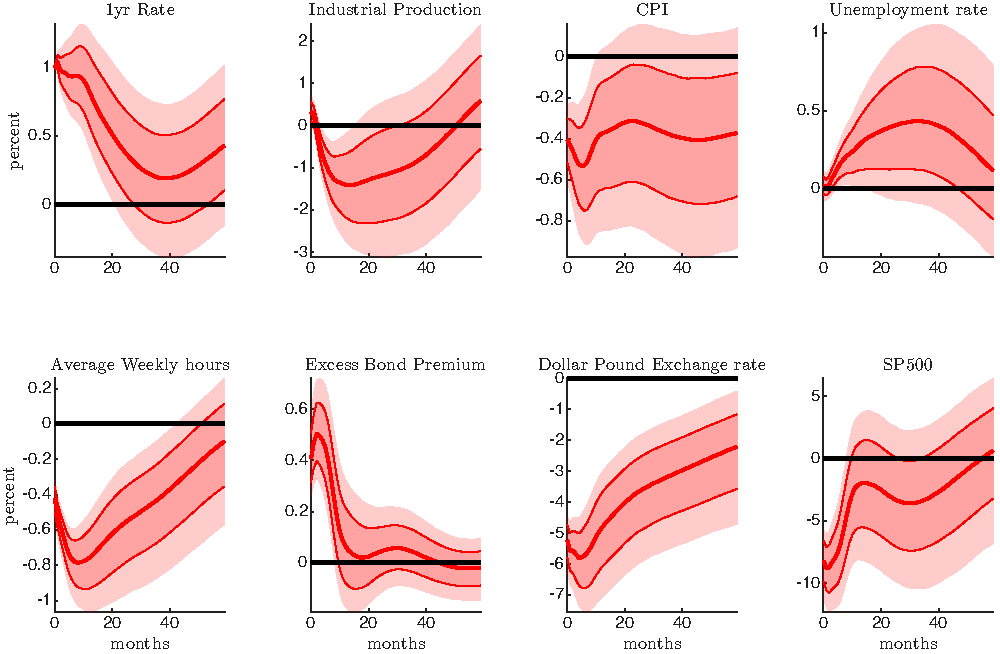
\includegraphics[width=\textwidth]{figures_final/figure1.pdf}
	\label{FF:aggregate:IRF}
    
	{\footnotesize \textit{Notes:} This figure depicts the impulse responses to a monetary policy tightening shock. From top left to bottom right: one year government bond yield; industrial production; consumer price index; unemployment rate; aggregate hours worked; excess bond premium; {\color{black}UK-US exchange rate}; S\&P500. Dark (light) red areas 68 (90)\% confidence sets. \par}
\end{figure}


The top panel of figure \ref{FF:disaggregate:IRF} shows our main result, that is the response of 'actual' hours worked for individuals at different slices of the earning distribution after a monetary policy tightening. %'Actual' hours worked are the self-reported hours of work which include overtime in the first job and possibly other jobs. 
For individuals above the 20th percentile of the earning distribution the impulse response of hours worked is qualitatively similar to the aggregate. %There is a persistent decline in aggregate hours after the monetary contraction. F
Hours fall persistently in the range of 0.5 to 0.8 percent at their trough in the middle 60 percent of the earning distribution, i.e. earnings between the 20 and 80 percentile. Hours worked also decline for the high income individuals albeit the peak effect is smaller, i.e. about 0.3 percent, and more short-lived.
In contrast, hours display a persistent increase on the left tail of the wage distribution. The peak response of hours occurs at about six month horizon and is estimated to increase by 1 percent.
Interestingly, the responses are more volatile on the left side of the earning distribution. The bottom panel of figure \ref{FF:disaggregate:IRF} reports the response of hours worked for households {\color{black}at the left tail of the wage distribution by varying the cut-off threshold.}
%in a finer slice of the wage distribution. 
In particular, the horizontal axis reports different percentiles of the wage earning distribution and the vertical axis the responses of hours worked after the shock for an income group below a certain percentile. {\color{black}Red (blue) lines and areas report the point and confidence sets two years (six months)  after the shock.} From this figure we can conclude that in the left tail of the income distribution a monetary policy tightening causes individuals to work more hours.

%below the 20th percentile of the wage (income) distributions obtained using the CPS survey and compares it with the average response of hours in the remaining groups above the 20th percentile and aggregate hours constructed from the CPS survey.

\begin{figure}[ht!]
	\caption{Distribution of responses to a monetary policy shock.}
	\centering
    %[trim=left bottom right top, clip]
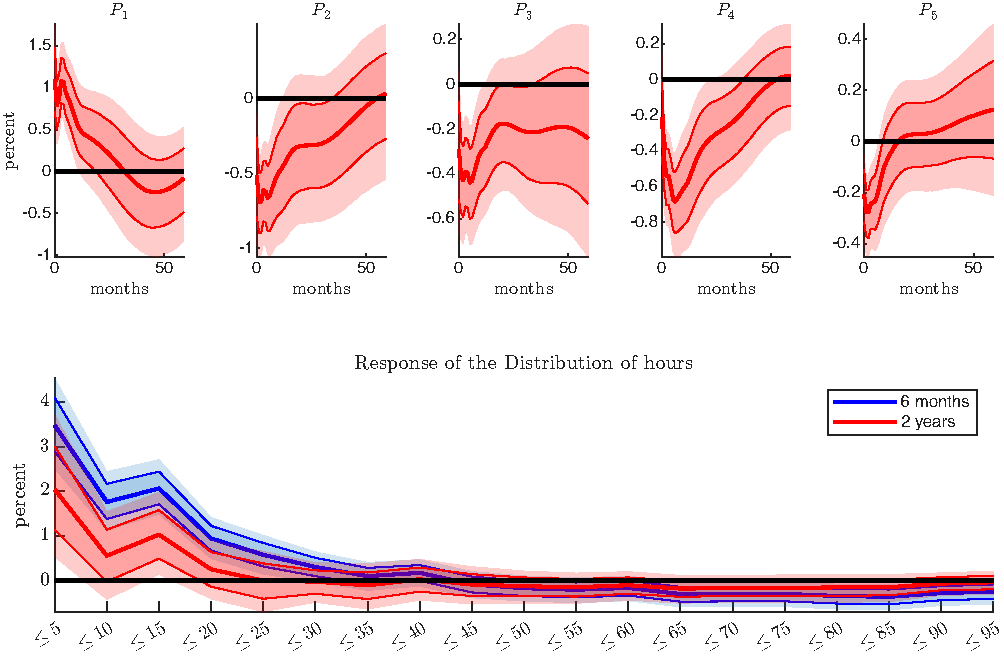
\includegraphics[width=0.9\textwidth,trim = 2cm 4.1cm 2cm 3.8cm]{figures_final/figure2_6.pdf}
	\label{FF:disaggregate:IRF}
    
	{\footnotesize \textit{Notes:} This figure depicts the impulse responses to a monetary policy tightening shock. Dark (light) red areas 68 (90)\% confidence sets. \par}
\end{figure}


\paragraph{Importance of the tail}

To have a sense of the importance of the response of hours worked of low- and moderate- income individuals for aggregate quantities we looked at different statistics. First, we computed the proportion of the variance of hours explained by the left tail, up to 20th and up to the 30th percentile of the wage distribution. The former (20th percentile) explains 16 percent of aggregate hours worked and 27 percent of the growth rate of aggregate hours, respectively; the latter (30th percentile) explains 29 percent of aggregate hours and 44 percent of the growth rate of aggregate hours. Second, we constructed an aggregate measure of hours worked based on CPS data and an alternative aggregate measure of hours worked which excludes the bottom 20 percent of the wage distribution. Figure \ref{FF:counterfactual:IRF} reports the responses of hours worked for the first quintile of the earning distribution (first panel), the aggregate measure of hours worked constructed using the CPS data (second panel) and the alternative aggregate measure of hours worked which excludes first quintile of the earning distribution (third panel). The response of the counterfactual (third panel) measure is 50 percent larger than the actual aggregate one (second panel). This suggests that the response of low-income individuals plays a non-trivial role in shaping the aggregate labor market outcomes and in particular in dampening the response of aggregate hours to a monetary policy shock.  

\begin{figure}[ht!]
	\centering
	\caption{Impulse responses to a monetary policy shock.}
    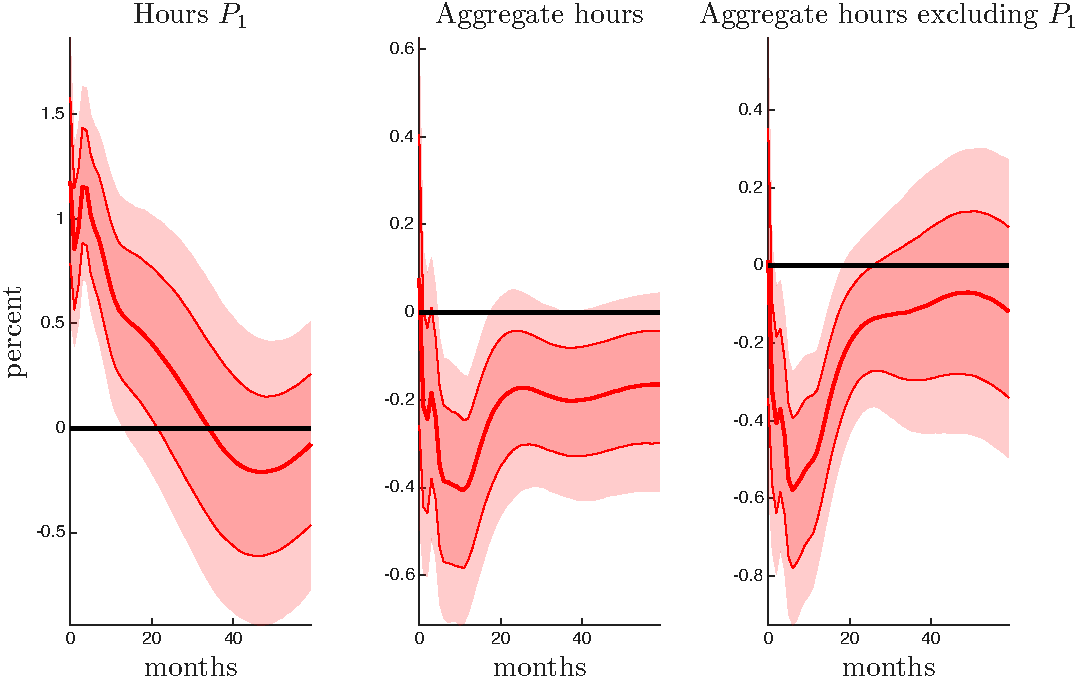
\includegraphics
    [width=0.85\textwidth,trim = 1cm 9cm 1cm 9cm]{figures_final/figure3.pdf}    %[width=6.5in,height=2.5in,scale = 0.50, clip=true,trim = 0cm 10cm -0.5cm 11cm]{figures_final/figure3.pdf}
	\label{FF:counterfactual:IRF}   
    
    {\footnotesize \textit{Notes:} This figure depicts the impulse responses to a monetary policy tightening shock. The left panel reports the responses of hours worked for the first quintile of the earning distribution, the cental panel the aggregate measure of hours worked using the CPS data, and right panel the alternative aggregate measure of hours worked which excludes first quintile of the earning distribution.  Dark (light) red areas 68 (90)\% confidence sets. \par}
\end{figure}

%An alternative way to organizing this information is to decompose the response of total hours worked to a monetary shock as the sum of employment multiplied by hours per worker for every income quantile. In figure \ref{RR:decomp:IRF}, we decompose the median response of aggregate hours worked (black line) after a monetary policy tightening into two components, the median amount of hours worked by individuals in the first income quintile of the earning distributions (violet bars) and the response of hours worked by workers with higher earnings (yellow bars); the sum of the bars coincides with the aggregate response. In the short run (first year and half), the response of the left tail significantly dampens the effect of the monetary tightening leading to milder contraction in hours worked relative to the case where the response of the low- and moderate- income individuals is neglected or zeroed. 

The extent to which this milder contraction in labor supply translates into less amplification of other variables (especially inflation)  is less clear. For answering the latter we need to construct an hypothetical counterfactual economy without the left tail of labor supply.
The empirical model does not allow to run such counterfactuals. The structural model presented in section \ref{T:Theory} can shed some light on this point. %Specifically, we consider different calibrations of a heterogeneous-agent New Keynesian (HANK) model where we vary the strength of the left tail of the labor supply response to monetary policy shocks, matching the heterogeneity documented empirically, and where inflation is linked to economic activity via the New Keynesian Phillips curve. We also compare these outcomes to a HANK model with homogeneous labor supply. By doing so, we quantify the macroeconomic implications of heterogeneity in labor supply, particularly focusing on the implications for the steady state, the transmission mechanism of monetary policy and on the the central bank's sacrifice ratio, defined as the output cost of reducing inflation.

%\begin{figure}[ht!]
%	\caption{Decomposition of aggregate hours worked.}
%	\centering
%	\includegraphics[width=\textwidth]{figures_final/decom.pdf}
%	\label{RR:decomp:IRF}
%	{\footnotesize \textit{Notes:} This figure decompose the median response of aggregate hours worked (black line) to a monetary policy tightening in terms of the response of the different percentiles of the income distribution. \par}
%\end{figure}

%\subsection{Composition Effects}
\paragraph{Composition Effects}
A potential concern about the empirical evidence presented earlier is that the observed increase in hours worked among low-income individuals following a monetary tightening may reflect composition effects. For instance, if part-time or low-hour workers are more likely to exit employment during downturns, average hours could rise mechanically even if individual labor supply remains unchanged. To address this concern, we first restrict the sample of our analysis to full-time workers.\footnote{For this exercise we use the  \href{https://cps.kansascityfed.org/}{Kansas Fed} extract of the CPS by setting the variable lfdetail76 equal to either $1$ or $2$.}  Figure \ref{fig:t:hours_full} displays the response of hours worked for different income levels. Removing part-time workers does not invalidate our main findings and hours increase at the left tail of the earnings distribution after a monetary contraction. 

\begin{figure}[ht]
    \centering
    \caption{Responses of hours for full-time employees}%
%[trim=left bottom right top, clip]
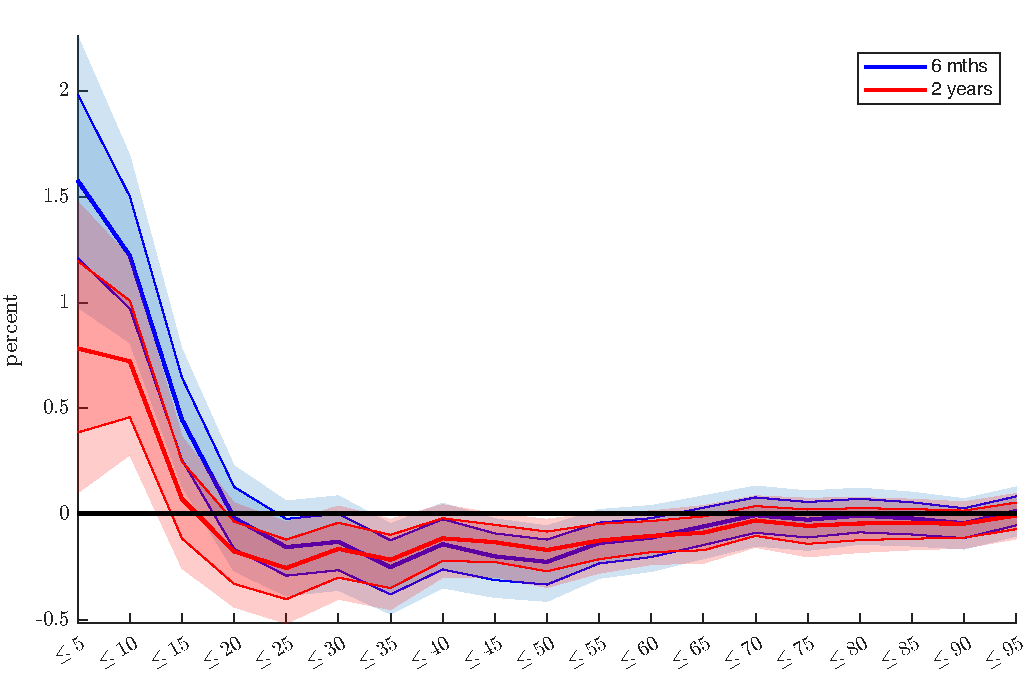
\includegraphics[width=0.7\textwidth,trim = 2cm 4cm 2cm 4cm]{figures_final/figure_ft_2.pdf}
    \label{fig:t:hours_full}   
    
{\footnotesize \textit{Notes:} This figure depicts the impulse responses to a monetary policy tightening shock. Dark (light) red areas 68 (90)\% confidence sets. \par}
   \end{figure}

Up to now our empirical analysis is constructed using a repeated cross-section which %might be more prone to errors due to changes in the composition and other confounding errors. 
even controlling for part- and full-time workers might still be prone to composition effects. 
To rule those out, we leverage the panel dimension of the CPS constructed by the Kansas City Fed (\href{https://cps.kansascityfed.org/}{https://cps.kansascityfed.org/}) and track changes in hours worked at the individual level. Specifically, we compute the change in hours between month $t$ and $t+12$ and use its average within income groups as the dependent variable in a FAVAR framework. This approach mitigates composition concerns inherent in cross-sectional averages.

\begin{figure}[ht!]
	\centering
    \caption{Distribution of responses of the growth rate of hours worked and of employment after monetary policy tightening.}
%	\centering\includegraphics[width=\textwidth]{figures_final/test3}
	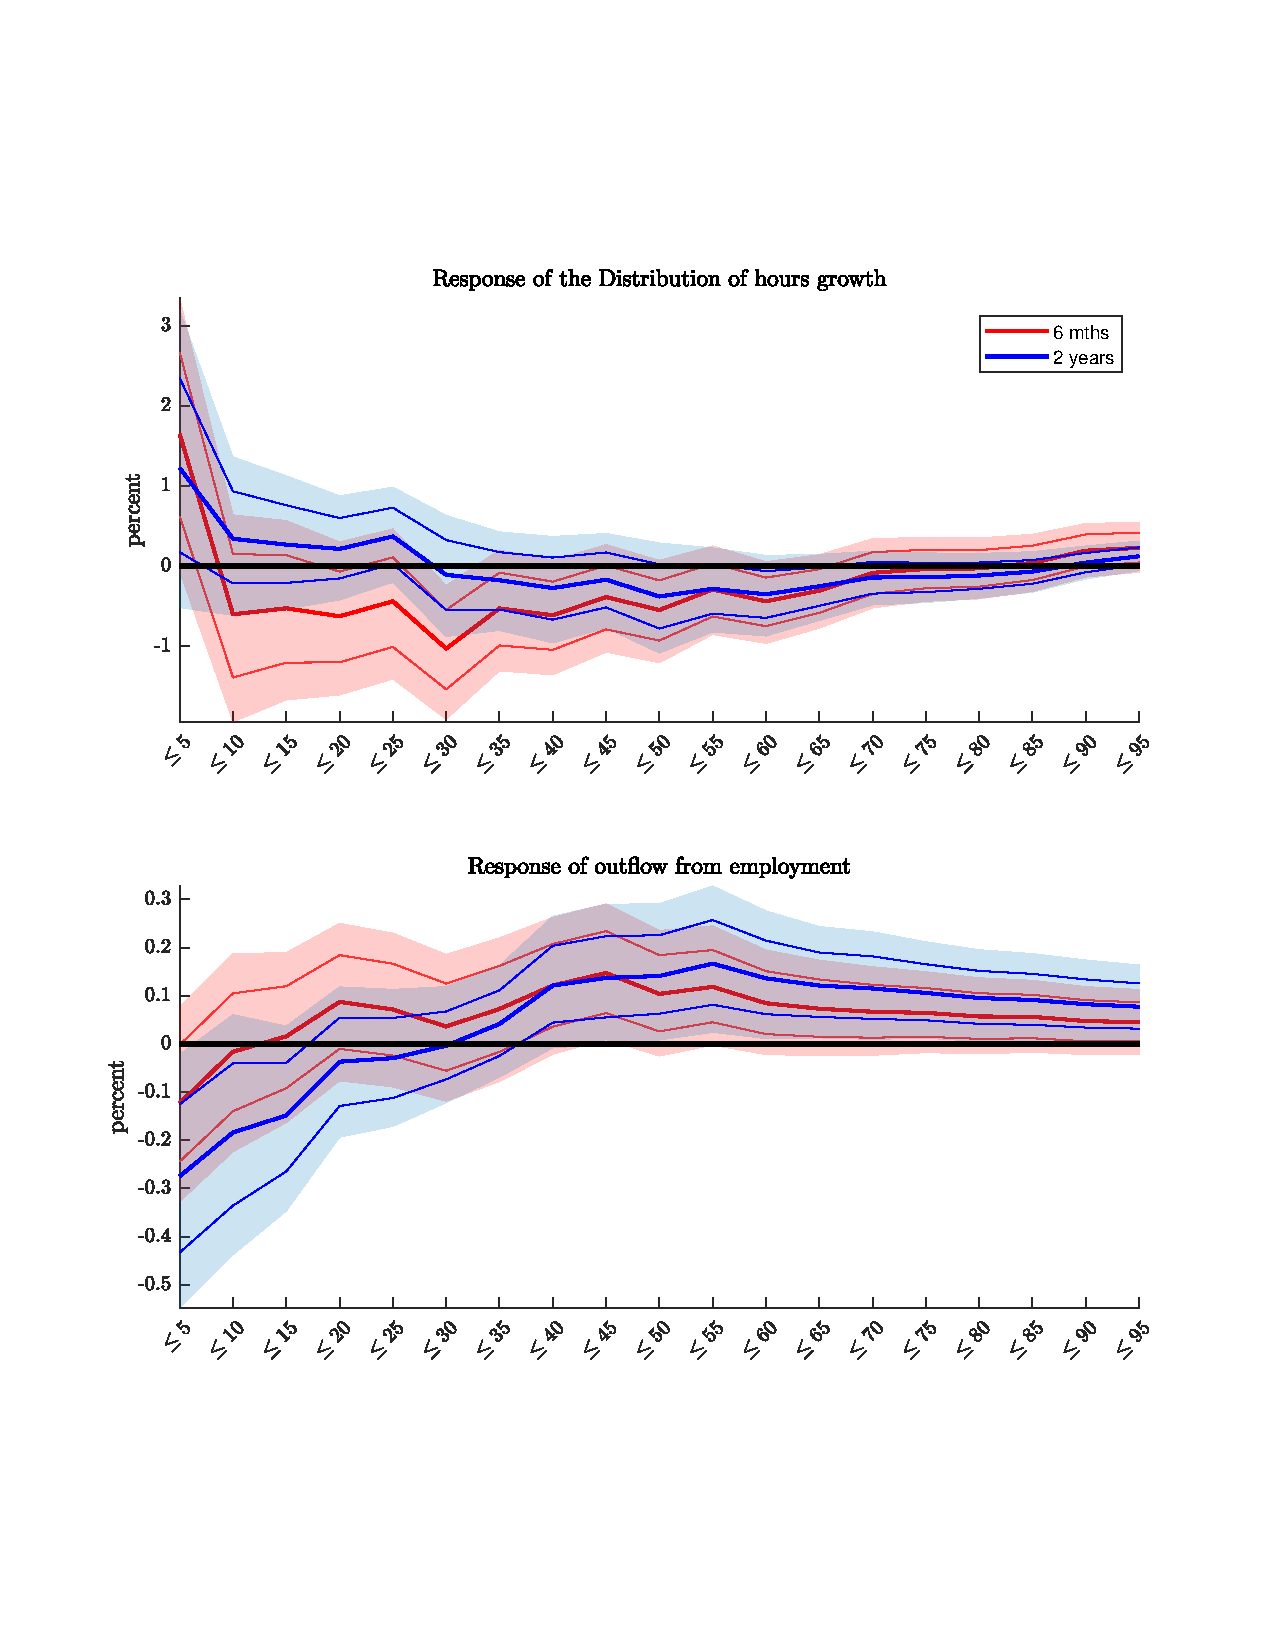
\includegraphics[width=0.9\textwidth,trim = 2cm 4cm 2cm 3.8cm]{figures_final/figure4_6.pdf}
	\label{FF:panel:IRF}
    
	{\footnotesize \textit{Notes:} The top panel depicts response of the growth rate of hours worked growth six months (red) and two (blue) years after the shock using the panel version of the CPS. The bottom panel depicts response of the outflows from employment six months (red) and two (blue) years after the shock using the panel version of the CPS. Shaded areas (solid lines) 68 (90)\% confidence sets. \par}
\end{figure}


The top panel of Figure \ref{FF:panel:IRF} shows the growth in hours worked six months (red) and two years (blue) post-shock, across the income distribution. Despite wider confidence intervals, the results support our main finding: low-income individuals increase their hours worked in response to contractionary policy. The bottom panel of Figure \ref{FF:panel:IRF} reports employment outflows\footnote{See footnote \ref{foot:empl} and Appendix \ref{App:Data:US:CPS} for details.} over the same horizon. While outflows rise for middle- and high-income groups, they decline for low-income individuals, indicating stronger job attachment in the lower tail of the distribution. 
These findings confirm that both intensive and extensive labor supply margins respond to monetary shocks, but in income-dependent ways. In the next sections, we interpret these patterns through the lens of theory.

\paragraph{Supply and demand factors}
%The countercyclical labor supply response at the bottom of the income distribution emerges from the interaction between household labor supply and firm labor demand. For middle- and high-income groups, both real wages and hours worked decline, consistent with falling labor demand (not shown here and reported in figure \ref{FF:wages:IRF} of the online appendix). In contrast, among low-income individuals, hours increase even as real wages fall--suggesting labor supply effects dominate.
%The countercyclical increase in labor supply among low-income workers reflects the interplay between household labor supply and firm-level labor demand. For middle- and high-income individuals, both real wages and hours worked decline following a monetary tightening, consistent with weaker labor demand (see Appendix Figure \ref{FF:wages:IRF}). In contrast, for workers in the lower part of the income distribution, hours increase despite falling real wages--suggesting that income effects on labor supply are the dominant force.
The countercyclical increase in labor supply among low-income workers reflects the interplay between household labor supply and firm-level labor demand. For middle- and high-income individuals, both real wages and hours worked decline following a monetary tightening, consistent with a leftward shift in labor demand. In contrast, among low-income workers, we observe rising hours despite falling real wages-indicating that income effects on labor supply dominate in this group. This pattern of negative comovement between wages and hours is suggestive of supply-side forces at play, as discussed in \citet{katz1992changes}, where such comovement typically reflects movements along a downward-sloping labor demand curve in response to shifts in labor supply. The responses of real wages at different income percentiles are reported in the Appendix \ref{A:realwages} figure \ref{FF:wages:IRF}. 

\paragraph{Sectors and education}
%We also explore sectoral heterogeneity. Most low-income workers are employed in wholesale and retail trade, leisure and hospitality, and education and health services (not shown here and reported in figure \ref{ind} of the online appendix). These sectors show pronounced income effects in labor supply responses.\footnote{See Figure \ref{irf_ind} in the online appendix.}

%Lastly, education moderates the strength of income effects. Low-income, non-college-educated individuals exhibit a larger increase in labor supply after monetary tightening than their college-educated peers (not shown here and reported in figure \ref{college} of the online appendix).

We further explore the heterogeneity behind this pattern by disaggregating responses by industry and education.\footnote{For more details see appendix \ref{A:ind_edu}.} Low-wage workers are largely employed in sectors such as wholesale and retail trade, leisure and hospitality, and education and health services (Appendix Figure \ref{ind}). Within these sectors, we observe clear positive responses of hours worked after a monetary contraction, especially at the bottom of the wage distribution (Appendix Figure \ref{irf_ind}).

Educational attainment also plays a role. Low-income, non-college-educated individuals exhibit a larger increase in labor supply after monetary tightening than their college-educated peers suggesting that education moderates the strength of income effects (Appendix Figure \ref{irf_educ1}).


%While non-college-educated individuals make up the majority of the left tail, a non-trivial share of low-wage workers has at least some college education (Appendix Figure \ref{college}). The increase in hours worked following a tightening is concentrated among non-college individuals, suggesting that stronger income effects in this group are a key driver of the aggregate response (Appendix Figure \ref{irf_educ}).


%The increase in hours worked at the bottom of the wage distribution after a monetary policy tightening could be the result of composition effects in the group of low- and moderate-income individuals. In particular, people working part time or fewer than 40 hours per week could be laid off during a monetary policy tightening cycle; thus, the average hours worked in this group could increase mechanically because these individuals drop off the sample. Hence, the increase in the hours worked observed in the previous section could be partly driven by composition effects as opposed to an increase in the labor supply. 

%To address this concern we considered the panel dimension of the CPS, constructed by the Kansas City Fed (\href{https://cps.kansascityfed.org/}{https://cps.kansascityfed.org/}). Using the CPS panel, we look at whether individual people change their hours worked in response to the shock. In particular, we construct the ''change in hours between month $t$ and $t+12$'' at the individual level, then use the average of that variable in a specific income group as the dependent variable in FAVAR. By focusing on the panel dimension, one removes any possible composition effects that could arise in the cross-section averages. 

%The top panel of Figure \ref{FF:panel:IRF} depicts response of the growth rate of hours worked growth six months (red) and two years (blue)  after the shock across the earning distribution using the panel version of the CPS. While there is less precision in the estimates, the results suggest that the main result of the paper is not overturned by compositional effects. In particular, we find that the low-income individuals tend to work more in response to a monetary contraction. The bottom panel of Figure \ref{FF:panel:IRF} reports the outflow of workers from employment the previous year to either unemployment or out of the labor force this year. The figures shows that, while in central and right portion of the income distribution a monetary policy contraction increases outflows from employment, in the left tail of the distribution this outflow declines two years after the shock, suggesting that people in this group remain attached to their job. 

%In sum, both the intensive and the extensive margins of the labor supply respond to the monetary policy shock, but they do so differently depending on the income level of the household. In the next sections, we try to interpret this finding through the lens of the theory. 

%The countercyclicality of hours worked in the left tail of the income distribution observed in the data is an equilibrium outcome resulting from the interaction of households' labor supply forces and firms' labor demand factors.  We find that both real wages (relative prices) and hours worked (quantities) move in the same direction for the center and right part of the income distribution.\footnote{Real wages both in the aggregate and at different percentile of the income distribution decline, see figure \ref{RR:wages:IRF} in the appendix.} This pattern aligns well with a downward shift in labor demand. However, this force is not strong enough in low and moderate income individuals, where we find that real wages declines but hours worked increases. In this case, an increase in the labor supply seems to be the dominant force. 

%We studied also the response of hours worked across the income distribution in different sectors. Low income workers are employed in a variety of industries with the bulk employed in wholesale and retail trade, leisure and hospitality and education and health services, see figure \ref{ind} in the appendix. %Construction constitutes a relatively small proportion of the total.  Sectors with large fraction of low income individuals  (wholesale and retail trade, leisure and hospitality and education and health services) feature strong income effects.\footnote{See figure \ref{irf_ind} in the appendix.}

%Finally, education attainment influence the strength of income effects. In fact, low income non-college workers tend to increase their labor supply more to monetary policy tightening compared to their peers with college educations.\footnote{See figure \ref{college} in the appendix.} 



%\todo[inline]{More robusntess? Sectoral stuff?}

%\subsection{Response of aggregate and dis-aggregate variables}

%The top panel of Figure \ref{f:IRF:1} shows the response of some key aggregate variables to a contractionary monetary policy shock in the US. The results are obtained using the monthly FAVAR which includes data on the distribution of hours from the CPS. The bottom panel reports the response of average hours worked for households below the $20^{th}$ percentile of the wage (income) distributions obtained using the CPS survey and compares it with the average response of hours in the remaining groups above the $20^{th}$ percentile and aggregate hours constructed from the CPS survey.\footnote{The responses of hours from the CEX survey are reported in the Appendix and discussed in the robustness section \ref{robustness} }

%\begin{figure}[h!]%
%\centering %trim=left bottom right top, 
%\includegraphics[width=\textwidth,trim=1cm 7cm 1cm 6cm]%
%{figures_final/Figure1_N}%
%\caption{Responses of selected variables to a contractionary monetary policy shock in the US normalized to a 1 percent increase in the one-year interest rate. The response of hours is weighted by the share of total hours in each percentile group. The response above the $20^{th}$ percentile is the weighted mean of the response of average hours in $20^{th}-40^{th}$, $40^{th}-60^{th}$, $60^{th}-80^{th}$ and above the $80^{th}$ percentiles. For each variable, we report the median IRF and 68\% bands. Except for aggregate hours for which we report only the median IRF.}
%\label{f:IRF:1}%
%\end{figure}

%The peak decline in output is about $3$ percent and CPI falls by $0.7$ percent. Stock market prices react negatively, with a peak response of around $13$ percent. Figure \ref{F:App:FAVAR:Macro:US} in appendix \ref{App:FAVAR:IRF} displays the response of selected macroeconomic and financial variables from the FAVAR models. The monetary contraction is associated with an increase in the unemployment rate, a fall in housing starts, and the real money supply. There is an increase in short-term interest rates, financial conditions deteriorate, and the exchange rate appreciates. In short, these results accord well with theory.


%The bottom panel of Figure \ref{f:IRF:1} shows our main result. There is a persistent decline in aggregate hours after the monetary contraction. For individuals above the $20^{th}$ percentile of the wage distribution, the impulse response is similar to the aggregate. Hours fall by $0.7$ percent at their trough. In contrast, hours display a persistent increase on the left tail of the wage distribution. The peak response of hours occurs at about the $2$ year horizon and is estimated to be an increase of $0.3$ percent. 

%Finally, the increase in hours worked induces an increase in the labor income; the %latter, however, does not rise more than hours worked suggesting a moderate decline in %hourly wages and therefore pointing towards an income effect driving the response of %hours in the left tail. These effects are shown in Figures % \ref{F:App:FAVAR:CEX:IRF:hours} and \ref{F:App:FAVAR:FES:IRF:hours} in the appendix.
 %In these figures, one can appreciate that the responses of the households in the 20 %percentile of the income distribution are significantly more volatile than the rest of %the population, both in the US and in the UK.

%So far we have arbitrarily chosen a cutoff percentile at 20 percent. In the next section, we look across the whole earnings distribution to check precisely where this threshold lies.


%\clearpage

%\subsection{Income effect on Labor Supply}\label{E:IE_LS}

%In this section, we present the results by running a set of empirical models. %Instead of sorting households into 5 bins of gross income, 
%We split the population into two groups, with average earnings below or above a certain percentile $J$, $P_{\leq J}$ and $P_{>J}$, respectively. We repeat the estimation of the FAVAR for $J = 5, 10, ..., 95$. In Figure \ref{f:IRF:2:US} we show the response of hours worked by individuals below a certain earnings threshold ($P_{\leq J}$) to a monetary policy tightening in the US for different thresholds ($J$) and different horizons.\footnote{Appendix \ref{App:3d} presents the full three-dimensional IRFs for hours worked, labor income and hourly wages.}

%The estimated response of hours confirms the results presented in the previous section, where we identified a portion of the population that increased their labor supply after a monetary-induced negative demand shock. The estimated model suggests that hours increase for individuals below the $20^{th}$ percentile after a contractionary shock at the one-year horizon. The response is negative towards the right tail of the earnings distribution, with the decline estimated to be statistically different from zero at the three-year horizon.
%The estimated response of hours from the CEX-based model is more volatile but suggests a similar conclusion. Hours increase for households below the $30^{th}$ percentile. In cumulative terms, the impact of the contractionary shock is negative towards the right tail of the income distribution.\footnote{In the CEX we observe a non-monotoning pattern. For the group below the 5 percent ($P_{\leq J}$), we see a decline in hours. However, this effect is short-lived (disappears after one year) and it is not present in the results from the CPS.}

%The increase in hours worked by households with low earnings could be the result of two mechanisms: more people at the bottom of the earning distribution enter the labor market (extensive margin), or employed people work longer (intensive margin). %\todo[inline]{Here we jump directly to income effect without discussing the other mechanisms we mention in the intro. We have two options: 1) add something like in the intro or 2) remain agnostic for the whole empirical evidence part and then add something at the end explaining that while we do not have data to distinguish between different stories we focus on the income effect on labor supply.} 
%Since the unemployment rate for low- and moderate-earnings individuals tends to increase after a monetary contraction --see the bottom right panel of Figure \ref{f:IRF:2:US}-- we can rule out large movements in the extensive margin. Hence, after a monetary-induced negative demand shock, low-earnings individuals who remain in the labor market tend to work longer hours. 
%The estimates of the exact magnitude of the labor supply increase and the precise threshold are difficult to pin down and depend on the survey considered. However, as we mentioned, these surveys are designed by construction to measure different patterns and behaviors.
%Low- and moderate-earnings households tend to explain non-negligible fractions of the variance of total hours worked and this fraction is larger than the analog for consumption. In the CPS survey, the cross-sectional variance of total hours worked explained by the bottom 30 percent of the labor income distribution ($P_{<30}$) is around 22 percent.\footnote{ 
%In the CEX survey, the same statistic is 23 percent. %the portion of consumption variance explained by the same group is smaller at 12 percent. }
%The labor supplied by the left tail of the labor income distribution represents also a relevant proportion of total hours worked in the economy. In the CPS, the average proportion of hours worked by the bottom 15 percent of workers across the labor income distribution is 15 percent.
%These numbers highlight an important difference between our work and the literature on consumption heterogeneity. The latter has stressed the importance of the \emph{wealthy} HtM households for matching the average marginal propensity to consume, empirically and theoretically (see e.g. \cite{KVW:14}). Here, our empirical analysis suggests that the labor supply heterogeneity does not arise for \emph{wealthy} HtM but rather for \emph{poor} HtM households, who appear to be crucial in driving labor supply heterogeneity following a monetary policy shock. Finally, we wish to emphasize that the labor market outcomes for low- and moderate- labor income households are significantly more volatile than for the rest of the population.
%}

%One concern with the benchmark results is that the impulse response of hours at the left tail reflects selection. That is, if the increase in the unemployment rate at the left tail of the earnings distribution is concentrated amongst part-time workers, then the increase in average hours could simply reflect the fact that more full-time workers remain in the sample after the shock. There are however several pieces of evidence that suggest that this is not the case. First, in our benchmark CPS sample we are able to construct unemployment rates for full-time and part-time workers, separately. As shown in the appendix, the monetary policy shock has a substantially larger impact on the unemployment rates of full-time workers at lower earnings quantiles than the corresponding rates of part-time workers. Second our benchmark results survive when we restrict the sample to individuals working full-time hours. Finally, as we discuss below, the response of hours at the left tail to general business cycle shock is \textit{negative}. This result goes against the argument that a substitution of full-time for part-time workers is driving our main result. 

%As discussed in the introduction, the countercyclicality of hours worked in the left tail of the income distribution observed in the data is an equilibrium outcome resulting from the interaction of households' labor supply forces and firms' labor demand factors. Isolating the channel responsible for our empirical finding is difficult with the data we consider and a combination of factors is more likely. One plausible rationale for the countercycliacal behavior of hours worked is a strong income motive pushing households with low incomes to work more hours. In the section where we discuss the theoretical models, we devote particular attention to this channel and study its implications for the transmission of monetary policy. 
%E.g., as the recession induced by a contractionary monetary policy increases the probability of becoming unemployed, households with limited income sources face larger risks; thus, to insure themselves against possible future income losses, members of such households might want to work more hours while they are still employed. Similarly, individuals who are close to their borrowing limits might desire to work more hours to meet their debt obligations when interest rates rise. Supply-side explanations suggest that when lacking buffer savings or nonlabor income sources, households with low incomes have less room to maneuver during tough economic times, and the labor supply allows them to smooth consumption along the business cycles. Alternatively, on the demand side, firms might lay off temporary or part-time workers and adjust the hour’s input by utilizing more of their existing labor force. 
%As a combination of factors is more likely, we focus our attention on the household supply channel and in particular on the 
%In sum, our empirical evidence suggests that after a monetary-induced negative demand shock, low-income individuals who remain in the labor market have a strong income effect on their labor supply. 



%Finally, it is important to highlight that, even considering just the intensive margin, labor income for individuals with low labor incomes is procyclical (see figure \ref{f:APP:li3d} in the appendix), in line with the evidence offered in \cite{BKM:2022} and \cite{HS:22}. This occurs because even if they work more hours, their average hourly earnings decrease relatively more, leading to a decline in their labor earnings. The focus of our analysis is precisely to isolate and study the intensive margin of employed individuals. 

%\todo[inline]{Here I am not sure if we should mention the implied response of labour income that I plot in figure D.5 in the appendix. I wanted to relate it to \cite{BKM:2022} and \cite{HS:22} but they look at the labor income of everyone, here we have the labor income of only the employed. If not we should remove figure D.5.. Everybody finds that labor income of poor people is pro cyclical (but they do have extensive and intensive margin) we find is countercyclical just for the intensive margin. }



%\begin{figure}[h!]
%    \centering
%            \includegraphics[width=\textwidth,trim=1cm 7cm 1cm 7cm]
 %           {figures_final/figure2_new}
  %          \caption{Impulse response of hours, earnings and the unemployment rate at different percentiles of the earnings distribution from the CPS. For each variable, we report the median IRF and 68\% bands.}
   %         \label{f:IRF:2:US}
%\end{figure}

% \clearpage
% \newpage

%======================================================================================
%\section{Theory}\label{T:Theory}

\section{Labor supply and heterogeneity}\label{T:Theory}

We now turn to a theoretical model to rationalize our empirical findings and assess their implications for the monetary policy transmission mechanism. We start from a general and stylized framework that clarifies the novel link between heterogeneous labor supply and monetary policy. Specifically, constrained agents facing tighter financial conditions tend to sacrifice leisure and increase labor supply to sustain their consumption in response to a decline in income.

Our empirical evidence, demonstrating that hours worked increase among households in the lower part of the income distribution after a monetary policy tightening, aligns with several potential theories. While the observed equilibrium outcome reflects both supply- and demand-side factors, the inverse movement of wages and hours worked--wages falling while hours increase--points predominantly toward a labor supply response driven by income effects. For this reason, in this section we focus the theoretical analysis on labor supply heterogeneity while assuming a standard labor demand side, modeled through a representative firm with homogeneous labor demand.

% We now turn to a theoretical model to rationalize our empirical findings and assess their implications for the monetary policy transmission mechanism. We begin with a general and stylized framework,\footnote{We thank an anonymous referee for suggesting this setup.} which clarifies the novel link between heterogeneous labor supply and monetary policy. Specifically, constrained agents sacrifice leisure to sustain consumption in response to declining income.

% Our empirical evidence on the response of the left tail of hours worked aligns with multiple theories. The observed equilibrium outcome reflects the interplay between household labor supply and firm labor demand. However, the inverse movement of wages and hours in the left tail--wages falling while hours increase--suggests that the dominant force is a labor supply response driven by an income effect, which we explore next.

% %While data limitations prevent us from discriminating empirically between each of those factors. However, it is most likely that our empirical evidence is driven by a combination of those factors.


\subsection{Income effects}\label{T:Intuition}
We begin by analyzing the household's problem in partial equilibrium, taking labor income as given, to highlight how the strength of the income effect on individual labor supply is shaped by two key forces: the curvature of the utility function and the tightness of the borrowing constraint.\footnote{We thank an anonymous referee for suggesting how to structure this section.}

A key feature in macroeconomic models determining household labor supply is the intratemporal optimality condition governing the trade-off between consumption and leisure. Let \( H_t \) denote hours worked at time \( t \), \( C_t \) consumption, and \( U(C_t,H_t) \) the household's utility function. With \( w_t \) as the real wage rate, this optimality condition is:
\begin{equation}
- \frac{U_h(C_t,H_t)}{U_c(C_t,H_t)} = w_t,
\end{equation}
where \( U_h \) and \( U_c \) are partial derivatives with respect to hours and consumption, respectively.

Households also face an intertemporal consumption decision summarized by the Euler equation (abstracting from uncertainty for now):
\begin{equation}
\frac{U_c(C_t,H_t)}{U_c(C_{t+1},H_{t+1})} = \beta (1 + r_t)(1 + \omega_t),
\end{equation}
where \( r_t \) is the real interest rate, affected by monetary policy, and \( \omega_t \) represents a wedge arising from borrowing constraints or other financial frictions. Typically, constrained households face a positive wedge (\( \omega_t > 0 \)), reflecting a higher marginal utility of current consumption. When the borrowing constraint binds, the Euler equation is replaced by a complementary slackness condition; in that case, the relevant link from monetary policy to constrained households operates through contemporaneous disposable-income and wealth (cash-flow) effects rather than intertemporal substitution.

Following a contractionary monetary policy shock that raises \( r_t \), the household's intratemporal optimality condition determines how hours worked adjust in response to changes in income and wages. The strength of this labor supply adjustment crucially depends on the curvature of the utility function over consumption. We assume preferences of the form:
\[
U(C_t, H_t) = \frac{C_t^{1 - 1/\sigma}}{1 - 1/\sigma} - \varphi \frac{H_t^{1 + \nu}}{1 + \nu},
\]
where \( \sigma \) denotes the elasticity of intertemporal substitution and \( \nu \) the inverse of the Frisch elasticity of labor supply.

A lower \( \sigma \) (corresponding to a more concave utility in consumption) implies that marginal utility reacts more strongly to income changes, amplifying the labor supply response when consumption declines. Households facing a negative income shock will then supply more labor to stabilize their utility. Conversely, a higher \( \sigma \) flattens the utility curve, making households less sensitive to fluctuations in income, and thus dampening the adjustment of hours worked.\footnote{See \cite{Bilbiie:2008}, who shows, in a two-agent NK model, how \( \sigma \) affects the sign of the response of the labor supply of hand-to-mouth agents.} 

Borrowing constraints (via \( \omega_t \) in the Euler equation) further magnify this effect by forcing some households to adjust labor supply more aggressively in response to changes in current disposable income and the real return on existing asset/debt positions. The borrowing limit directly affects the strength of this labor supply channel. A tighter borrowing constraint (or higher equilibrium debt levels) amplifies the sensitivity of labor supply to monetary policy shocks: when the real interest rate rises, higher debt repayments reduce disposable income, strengthening the income effect. Constrained households, unable to smooth consumption through borrowing, respond by increasing their labor supply to offset the higher financial burden.

In Appendix \ref{A:BSmodel}, we illustrate how these forces interact in a simple two-agent (borrower-saver) economy where borrowers face tighter borrowing limits and higher impatience relative to savers. We show analytically how borrowers' labor supply response after an interest rate increase depends directly on the EIS (decreasing in \( \sigma \)) and their borrowing limit (increasing in the net debt position).

Thus, both the EIS and borrowing constraints crucially shape the extent to which the labor supply of constrained households becomes countercyclical following monetary policy shocks, offering a clear theoretical interpretation in terms of labor supply of our empirical findings. 

% A key feature of many macroeconomic models is the household's intratemporal condition governing the trade-off between consumption and leisure. Let \( H_t \) denote hours worked at time \( t \), \( C_t \) consumption, and \( U(C_t,H_t) \) preferences over both. With \( w_t \) as the wage rate (normalized by the price of consumption), the optimality condition is:  
% \begin{align}
%     -\frac{U_h(C_t,H_t)}{U_c(C_t,H_t)} = w_t,
% \end{align}
% where \( U_h \) and \( U_c \) are the partial derivatives with respect to hours worked and consumption, respectively.  
% Households also face an intertemporal trade-off given by the Euler equation (we are abstracting from risk for now):  
% \begin{align}  
%     \frac{U_c(C_{t},H_{t})}{U_c(C_{t+1},H_{t+1})} = \beta(1+r_t)(1+\omega_t),  
% \end{align}  
% where \( r_t \) is the real interest rate, influenced by monetary policy, and \( \omega_t \) represents frictions such as borrowing constraints. Typically, constrained households have \( \omega_t > 0 \), implying higher marginal utility of consumption today than the one implied by a Euler Equation with $\omega_t=0$.  

% \todo[inline]{Note: I changed $\tau$ to $\omega$ for the wedge as I use $\tau$ for taxes later on.}
% Following a contractionary monetary policy shock that raises \( r_t \), the marginal utility of consumption increases. This can manifest as a rise in \( U_h \) (which increases \( H_t \)) or a decline in \( w_t \). The labor supply response depends on the relative strength of income effects (ie. the slope of the labor supply curve). If substitution effects dominate, households reduce labor supply. However, if income effects dominate, the labor supply increases. Moreover, these effects are stronger if the Euler equation wedge correlates with the real interest rate. As long as the increase in $r_t$ reduces the household income, the latter is typically the case for households on the borrowing limit or hand-to-mouth.\footnote{In the appendix we derive the aggregate intratemporal optimality condition with a two agents, savers and hand-to-mouth, model and derive the conditions under which the labor supply of hand-to-mouth agents increase after a monetary policy contraction.}  
% \todo[inline]{I am not convinced by this. }
In the next section, we move to a general equilibrium analysis and consider a standard one-asset heterogeneous agents New Keynesian model with staggered price setting. %We show how labor supply varies along the income distribution and quantify its dependence on the elasticity of intertemporal substitution (EIS) and the borrowing limit.


\subsection{Heterogeneous Labor Supply in HANK}\label{T:HANK}
The purpose of this section is to demonstrate that our empirical evidence aligns with the implications for heterogeneous labor supply responses in a standard HANK model. To do so, we use the one-asset HANK model with endogenous labor supply, as in \cite{ABRS21}.\footnote{The only difference with \cite{ABRS21} is that we abstract from government spending, given the focus on monetary policy here. Results are not affected by this choice.} The goal is to examine how different calibrations of the model affect the behavior of labor supply across the income and wealth distribution, and to compare the aggregate implications for the monetary transmission mechanism with and without heterogeneous labor supply responses in the model.
The main results are as follows:
(i) An off-the-shelf HANK model with heterogeneous labor supply and homogeneous labor demand can replicate our empirical findings on the labor supply response across the income distribution.
(ii) The main driver of the response at the lower end of the distribution is an income effect, stemming from falling wages and rising debt repayments. Moreover, the strength of this response is amplified by the curvature of the utility function in consumption and the tightness of the borrowing limit, further highlighting the importance of income effects.
(iii) The presence of labor supply heterogeneity lowers the real cost of disinflation, making it easier for the central bank to achieve its inflation target.
% The main results are the following: i) an off-the-shelf HANK model with heterogeneous labor supply and homogeneous labor demand can replicate our empirical findings on the labor supply response across the income distribution; ii) the most important driver of the response of the left tail of the labor supply is an income effect from falling wages and raising debts repayments; %Moreover the strength of the response at the lower end of the income distribution is driven by the curvature of the utility function in consumption and the tightness of the borrowing limit, pointing to the importance of income effects; 
% iii) the presence of labor supply heterogeneity lowers the real cost of disinflation, making it easier for the central bank to achieve its inflation target.


\subsubsection{One-asset HANK}
The model features a heterogeneous agents sector similar to \cite{MNS:2016}, coupled with a standard New Keynesian supply-side block.

\emph{Households}. There is a unit mass of ex-ante identical households who differ ex-post by their labor productivity \( e \) (``skill'') and asset holdings \( a \). For notational simplicity, we use the subscript \( i \) to denote household-level outcomes, instead of writing them explicitly as functions of state variables.

Skill \( e \) follows a time-invariant discrete Markov chain with \( n_e \) states, \( \mathcal{E} = \{e_1, e_2, \ldots, e_{n_e}\} \), and exogenous transition probabilities \( P(e^{\prime}, e) \). This introduces cyclical income risk in the model. The stationary distribution of \( P \) is denoted by \( \pi_e \). Average labor productivity \( \int_0^1 e_{i,t} \, di \) is invariant and normalized to 1.

We assume that \( P(e^{\prime}, e) \) discretizes a log AR(1) process:
\[
\log e_{i t} = \rho_e \log e_{i t-1} + \sigma_{\epsilon,e} \epsilon_{i t},
\]
with normal innovations \( \epsilon_{i t} \sim \mathcal{N}(0,1) \).\footnote{In Table \ref{tab:HANK_calib} we report the stationary cross-sectional dispersion \( \text{Std}(\log e) = \sigma_e \); given \( \rho_e \), the corresponding innovation standard deviation is \( \sigma_{\epsilon,e} = \sigma_e \sqrt{1-\rho_e^2} \) (for the baseline calibration, \( \sigma_{\epsilon,e}\approx 0.13 \)).} We use the Rouwenhorst method for discretization.

Households can freely choose the number of hours \( h \) they work, subject to an additively separable utility cost of working. Consumption, savings, and labor choices \( c \), \( a \), and \( h \) are the solution to the household's utility maximization problem, characterized by the following Bellman equation:
\[
\begin{aligned}
V_t\left(e_{i t}, a_{i t-1}\right) = \max_{c_{i t}, h_{i t}, a_{i t}} & \left\{ \frac{c_{i t}^{1 - \sigma^{-1}}}{1 - \sigma^{-1}} - \varphi \frac{h_{i t}^{1 + \nu}}{1 + \nu} + \beta \mathbb{E}_t V_{t+1}\left(e_{i t+1}, a_{i t}\right) \right\} \\
\text{s.t.} \quad & c_{i t} + a_{i t} = (1 + r_t) a_{i t-1} + w_t e_{i t} h_{i t} - \tau_t \bar{\tau}(e_{i t}) + d_t \bar{d}(e_{i t}) \\
& a_{i t} \geq \underline{a}.
\end{aligned}
\]

Households receive an hourly wage \( w_t \), pay taxes, and receive dividends from firm ownership according to incidence rules \( \bar{\tau}(e) \) and \( \bar{d}(e) \).\footnote{
This implies that skill \( e \) determines not only a household's income per hour worked, but also the amount of lump-sum taxes she must pay and the dividends she receives, both of which are distributed proportionally to \( e \).}

\emph{Firms}. A competitive final goods firm assembles its output using a CES production function \( Y_t = \left( \int_0^1 y_{j t}^{\frac{1}{\mu}} dj \right)^\mu \), giving rise to a standard CES demand system for the continuum of intermediate goods. These intermediates, in turn, are supplied by monopolists who produce using only labor, such that \( y_{jt} = Z_t h_{jt} \), and are subject to quadratic price adjustment costs a la \cite{Rotemberg:1982}:
\[
\psi_t\left(p_{j t}, p_{j t-1}\right) = \frac{\mu}{\mu-1} \frac{1}{2 \kappa} \left[ \log \left( \frac{p_{j t}}{p_{j t-1}} \right) \right]^2 Y_t.
\]
Here, \( Z_t \) denotes aggregate productivity that may be time-varying. In a symmetric equilibrium, gross inflation \( 1 + \pi_t = \frac{P_t}{P_{t-1}} \) evolves according to the Phillips curve:
\[
\log(1+\pi_t) = \kappa \left( \frac{w_t}{Z_t} - \frac{1}{\mu} \right) + \frac{1}{1 + r_{t+1}} \frac{Y_{t+1}}{Y_t} \log(1 + \pi_{t+1}),
\]
and dividends equal output net of labor and price adjustment costs: \( d_t = Y_t - w_t H_t - \psi_t \).

\emph{Policy}. Monetary policy sets the nominal rate on bonds according to a standard Taylor rule: 
\[
i_t = r^* + \phi \pi_t+\epsilon_t,
\]
where \( r^*_t \) is the economy's long-run ``natural rate'' and $\epsilon_t$ the monetary policy shock. The real interest rate in period \( t \) is determined by the previously set nominal rate and inflation so that:
\[
1 + r_t = \frac{1 + i_{t-1}}{1 + \pi_t}.
\]

The fiscal authority, in turn, issues a constant amount of government bonds \( B \) each period and collects the lump-sum taxes \( \tau_t \) already mentioned above. Since there are no other spending items (abstracting from government spending), it chooses the tax rate to cover its interest rate payments every period:
\[
\tau_t = r_t B.
\]

\emph{Market Clearing}. In an equilibrium, the following market clearing conditions must hold:
\begin{itemize}
    \item Asset market:
    \[
    B = \int_0^1 a_{it} \, di,
    \]

    \item Labor market:
    \[
    Y_t = H_t = \int_0^1 e_{it} h_{it} \, di,
    \]

	    \item Goods market:
	    \[
	    Y_t = \int_0^1 c_{it} \, di + \psi_t.
	    \]
	\end{itemize}

These in turn imply that aggregate household savings equal government-provided liquidity, labor demand equals supply in efficiency units, and the final good is used for consumption and price adjustment costs.\footnote{As is well known, price adjustment costs don't matter in linearized models.}


\paragraph{Calibration}
The model is solved using the \emph{sequence-space Jacobians} approach pioneered by \cite{ABRS21}.\footnote{See \cite{BayerLuetticke2020} for an alternative solution method.} For technical details, we refer the reader to their paper. The calibration is also mostly taken from \cite{ABRS21} and summarised in Table \ref{tab:HANK_calib}. The main difference from their calibration is that here we also choose $B$ to target a percentage of HTM agents in steady state of 20\%. This is to ensure a comparison across different models and/or calibrations keeping fixed the steady state proportion of constrained agents. The other difference is that, in the baseline calibration, we allow for some borrowing in equilibrium ($\underline{a}=-0.5$).\footnote{The implied $\beta$ and $\varphi$ are almost identical to theirs, while our calibration requires a lower amount of liquidity compared to their model, where they set $B=5.6$ and obtain MPC = 11\% and HTM = 17\%. All the results presented in this section do not change substantially if we use their original calibration.} This calibration implies an income-weighted aggregate MPC in steady state equal to 12.5\%.

\begin{table}[h!]
\centering
\begin{tabular}{@{}llcc@{}}
\toprule
\textbf{Parameter} & & \textbf{Value} & \textbf{Target} \\
\midrule
\multicolumn{4}{@{}l}{\textit{Households}} \\
$\beta$ & Discount factor & 0.98 & Asset market clearing \\
$\varphi$ & Disutility of labor & 0.78 & Labor market clearing\\
$\sigma$ & EIS & .5 & \\
$\nu$ & Inverse Frisch & 2 & \\
$\underline{a}$ & Borrowing constraint & -0.5 & \\
$\rho_e$ & Autocorrelation of earnings & 0.966 & \\
$\sigma_e$ & Cross-sectional std of log earnings & 0.5 & \\
\addlinespace
\multicolumn{4}{@{}l}{\textit{Firms}} \\
$\mu$ & Steady-state markup & 1.2 & \\
$\kappa$ & Slope of Phillips curve & 0.1 & \\
\addlinespace
\multicolumn{4}{@{}l}{\textit{Policy}} \\
$B$ & Bond supply & 3.84 & HTM = 0.2 \\
$\phi$ & Taylor rule coefficient on inflation & 1.5 & \\
\addlinespace
\multicolumn{4}{@{}l}{\textit{Monetary Policy Shock}} \\
$\rho_{\epsilon}$ & Persistence & 0.61 & \\
$\sigma_{\epsilon}$ & Standard Deviation & 0.0025 & \\
\addlinespace
\multicolumn{4}{@{}l}{\textit{Discretization}} \\
$n_e$ & Points in Markov chain for $e$ & 7 & \\
$n_a$ & Points on asset grid & 500 & \\
$\bar{a}$ & Upper limit on asset grid & 150 &\\
\bottomrule
\multicolumn{4}{@{}l}{\textit{Untargeted Steady State}} \\
MPC & \% aggregate Marginal Propensity to Consume & 12.5\% &\\
r  & quarterly real rate & 0.5\% & \\
H & effective aggregate labor supply & 1 & \\
\bottomrule
\end{tabular}
\caption{One-asset HANK calibration}
\label{tab:HANK_calib}
\end{table}




\paragraph{Rationalizing the empirical evidence} 

Mapping the discrete income states to their positions in the steady-state distribution reveals that both consumption and labor supply, on average, increase with income--consistent with empirical evidence. However, poorer households near the borrowing constraint tend to work more than richer ones due to stronger income effects and tighter liquidity.\footnote{See appendix \ref{A:HANK_SS} for details.}


\begin{figure}
    \centering
    \caption{Impulse responses to a 25 basis points Monetary Policy Shock}
    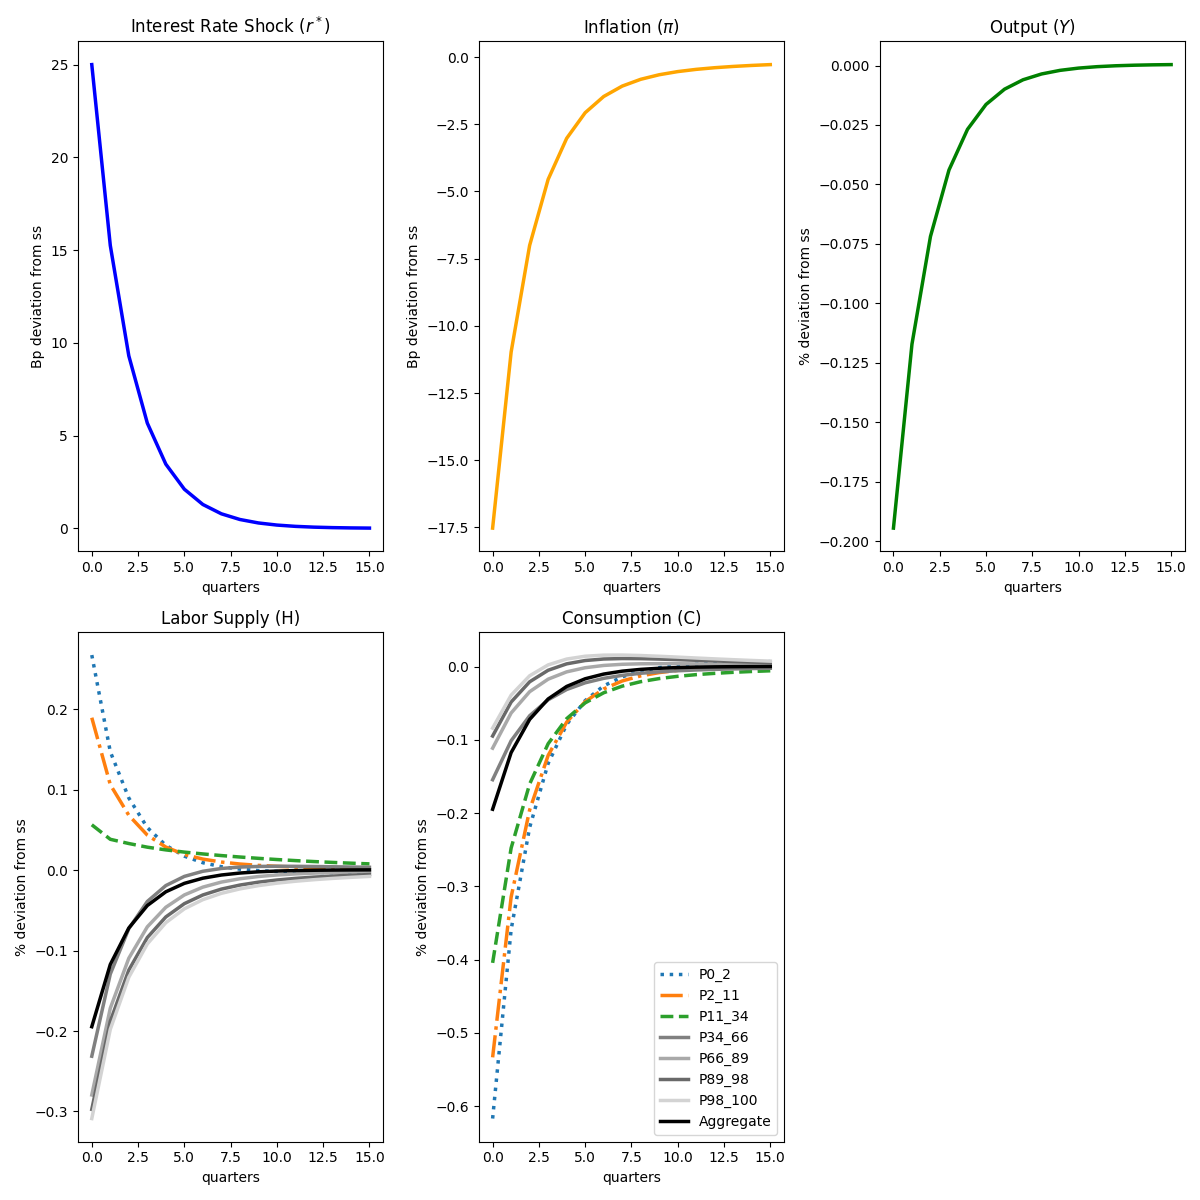
\includegraphics[width=\linewidth]{figures_final/baseline_IRFs_with_L_and_C.png}
    \label{fig:baseline_irfs}
\end{figure}


Figure \ref{fig:baseline_irfs} shows the impulse responses to a monetary policy tightening, assuming that $\epsilon_t$ follows an AR(1) process with persistence $\rho_{\epsilon}=0.61$ and standard deviation $\sigma_{\epsilon}=0.0025$. The upper panels display the dynamics of the interest rate shock, inflation, and aggregate output. The lower panels highlight heterogeneous labor supply and consumption responses across income groups.
Poorer households (e.g., P0\_2, P2\_11, and P11\_34) increase labor supply following the shock, consistent with a dominant income effect driven by tight borrowing constraints. In contrast, higher-income households reduce labor supply, reflecting standard substitution effects. Consumption falls across all groups but declines more sharply for lower-income households, as expected. 
These results demonstrate that an off-the-shelf HANK model is able to capture our empirical evidence on the heterogeneous labor supply behavior across the income distribution in response to a monetary policy shock. It is important to stress that, since the model features a representative firm, labor demand is homogeneous across agents. However, while the physical unit of labor is identical across households, effective labor supply differs due to heterogeneity in individual productivity.


Next, in order to assess how labor supply responses to monetary policy shocks vary across the income distribution, and to understand the role of key structural parameters, we perform a comparative exercise across different model calibrations. Specifically, we vary the two critical parameters identified in the previous section: the borrowing constraint (comparing $\underline{a} = 0$ - no borrowing allowed - with the baseline calibration $\underline{a} = -0.5$) and the EIS, which governs households' willingness to smooth consumption over time and the relative strength of the income and substitution effects on their labor supply.\footnote{Appendix \ref{A:HANK_PF} reports policy functions and IRFs for all calibrations.}



\begin{figure}
    \centering
        \caption{Impact Impulse Responses of Labor Supply Across the Income Distribution}
    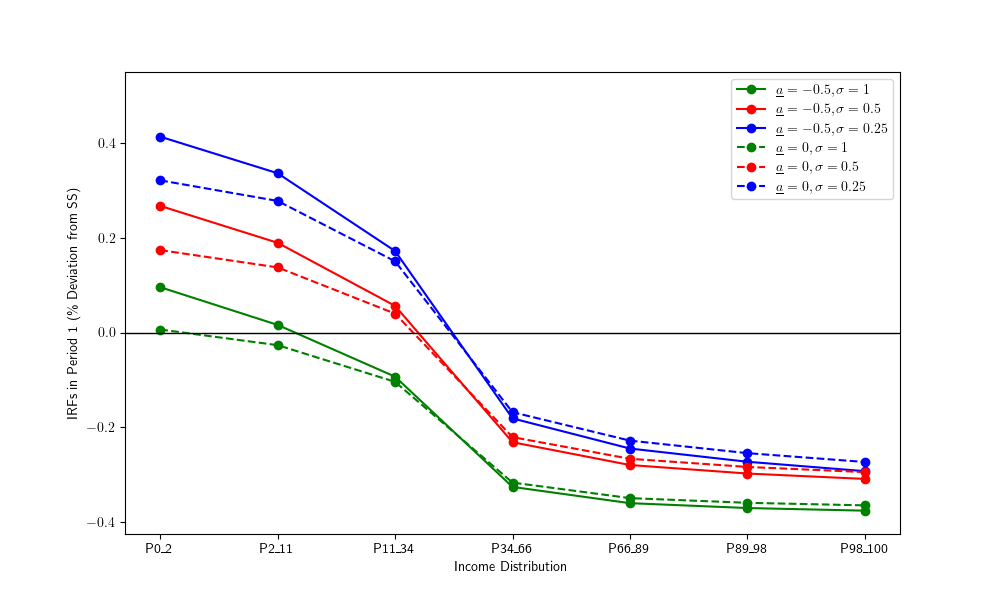
\includegraphics[width=\linewidth]{figures_final/labor_supply_models_across_income.png}
    \label{fig:labor_supply_models_across_income}
\end{figure}

By analyzing the impact impulse responses (IRFs) of labor supply across income groups under these alternative specifications, we aim to isolate how tighter borrowing constraints and the EIS interact with income heterogeneity to shape aggregate and disaggregate labor market dynamics following monetary policy shocks. Figure \ref{fig:labor_supply_models_across_income} plots the impact responses of labor supply for households across seven income groups (from P0\_2 to P98\_100), under the six different model calibrations. Solid lines correspond to the baseline borrowing constraint calibration $\underline{a} = -0.5$, allowing limited debt, while dashed lines represent a tighter borrowing constraint $\underline{a} = 0$ (no debt allowed). Different colors denote different values of the EIS: blue for $\sigma = 0.25$ (high income effect), red for $\sigma = 0.5$ (baseline), and green for $\sigma = 1.0$ (low income effect).

Across all models, except for the case $\underline{a}=0$ \& $\sigma=1$, we observe that the bottom income groups (P0\_2, P2\_11) increase their labor supply after a monetary tightening, while upper income groups (P34\_66 and above) reduce labor supply. Allowing for borrowing ($\underline{a} = -0.5$) amplifies the need for immediate labor adjustment, leading to higher increases in labor supply at the bottom compared to the no-borrowing case. Similarly, lower EIS (lower $\sigma$) amplifies labor supply responses at the bottom, as households are more willing to reallocate labor to smooth consumption. In contrast, when EIS is high ($\sigma = 1$), the labor supply responses are significantly muted across the distribution, especially among the lower-income groups. Overall, the interaction between borrowing constraints and EIS shapes the heterogeneous labor market adjustments following monetary policy shocks. Importantly, this figure shows that while a low elasticity of intertemporal substitution (EIS) is sufficient to induce a change in the sign of the labor supply IRFs for households in the left tail of the income distribution, allowing for a negative borrowing limit ($\underline{a} < 0$) is necessary to generate a larger magnitude of the (absolute value of) labor supply responses at the bottom of the distribution, in line with our empirical results.

\paragraph{IRFs decomposition} Contrary to the FAVAR, this model allows us to check what is driving the left tail of the labor supply response. To understand this, we decompose the total impulse responses into marginal contributions from individual channels. Specifically, we compute the Jacobians of household consumption with respect to the following inputs: the real interest rate ($r$), labor income ($w$), and transfers, defined as dividends ($\text{Div}$) minus taxes ($\text{Tax}$). Figure~\ref{fig:hetl_labor_decomp_combined} shows the decomposition of total effective labor supply (top left panel) in terms of these main channels. The top left panel of this figure reports the decomposition of the aggregate hours worked while the subsequent panels report the same decomposition for different percentiles of the income distribution. Labor income is the main driver of the decline in aggregate hours worked (yellow bars). A lower real hourly wage reduces the aggregate incentive to work. The real rate (blue bars), instead, pushes aggregate labor supply up during the first two quarters. In the SSJ decomposition, the $r$ input isolates the marginal effect of the real interest rate holding wages and fiscal flows (Div and Tax) fixed. This contribution reflects intertemporal-substitution effects for unconstrained households and contemporaneous cash-flow/wealth effects on existing asset and debt positions; for low-income/near-HTM households, the debt-service (cash-flow) channel is the key driver of the positive $r$ contribution. Transfers, defined as the difference between dividends and taxes, marginally affect the dynamics (red bars).

\begin{figure}[h!]
  \centering
  \caption{Decomposition of labor supply responses in HANK.}
  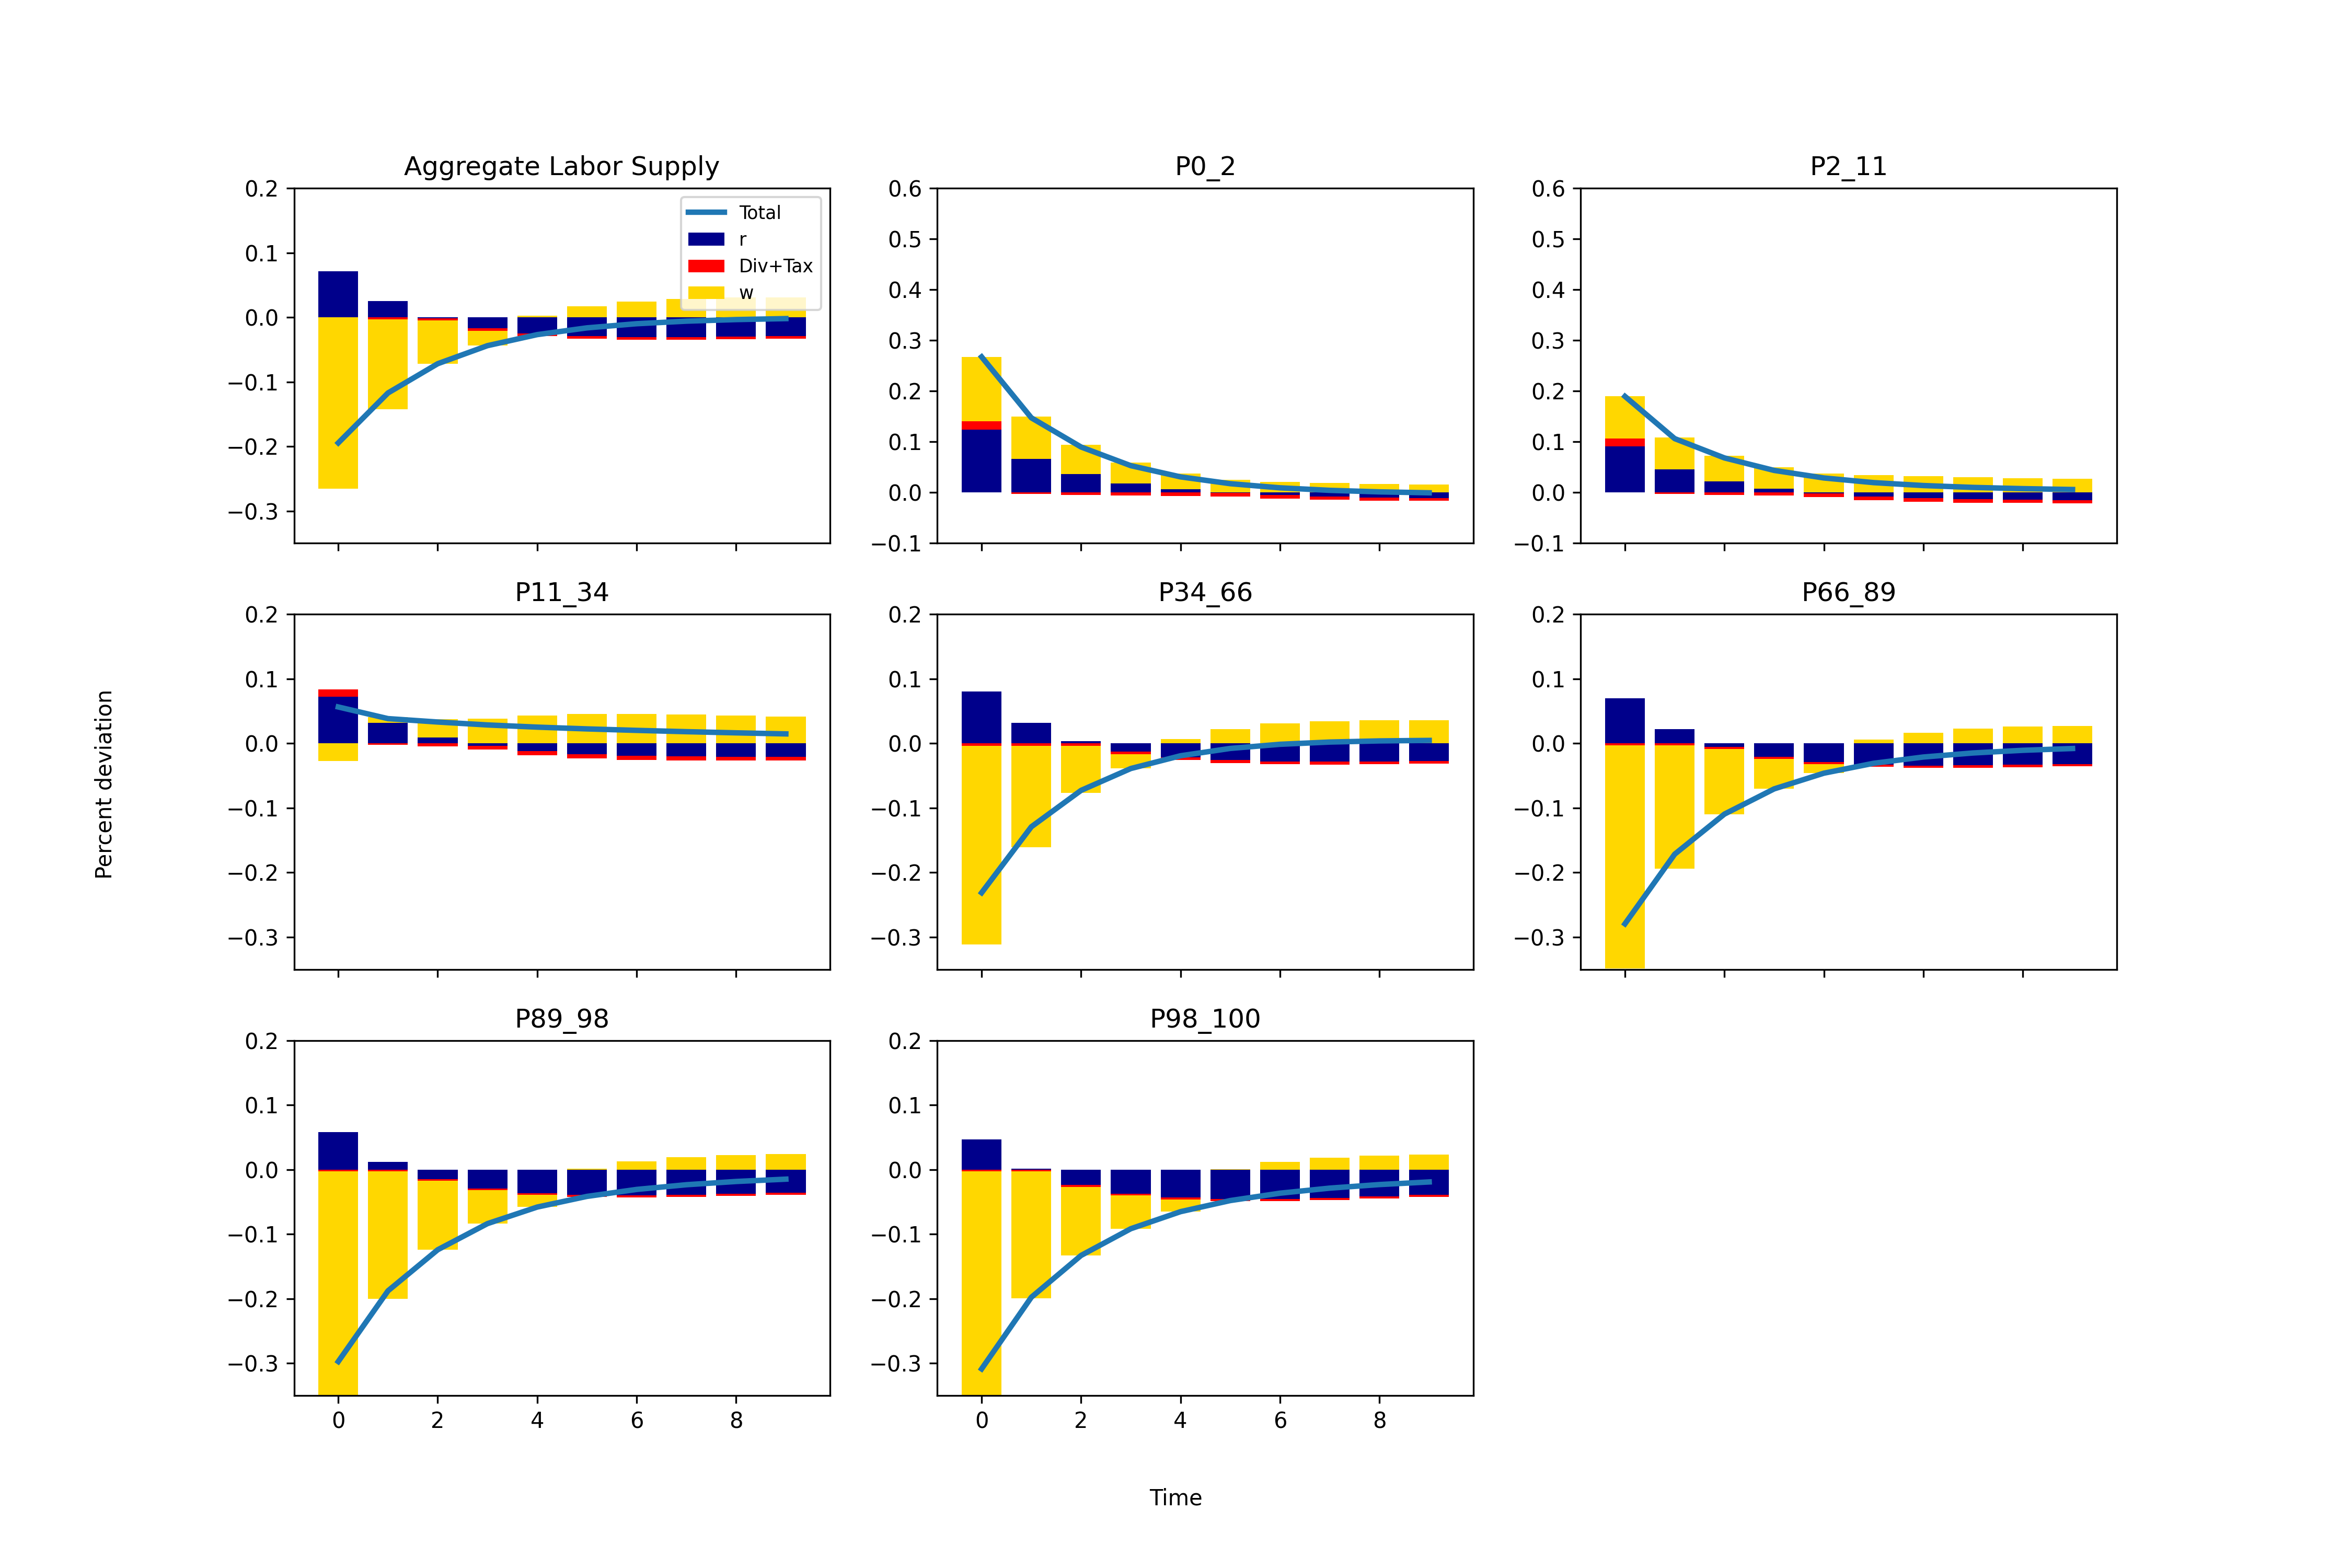
\includegraphics[width=1\textwidth]{figures_final/HANK_HetL_decomp_bins_H_comb.png}
  \label{fig:hetl_labor_decomp_combined}
\end{figure}

Now the question is, how does this picture change when we zoom in at the individual level? And what is the force behind the left tail of the labor supply? 
The other panels in Figure \ref{fig:hetl_labor_decomp_combined} answer these questions by plotting the decomposition of labor supply by each income state. First, we notice that the real rate channel on impact is stronger at the bottom of the income distribution, and it remains positive for more periods compared to agents in the middle to the top of the distribution. 
This is in line with the fact that the income effect from debt repayments is larger for poorer individuals. 
Moreover, the yellow bars flip sign at the bottom, pointing towards another income effect coming from labor income. 
For poor households, the income effect of a lower hourly wage dominates the substitution effect. Hence, in line with the simple analytical discussion presented at the beginning of this section, these results show that the combination of borrowing constraints and strong income effects on labor supply are responsible for matching our empirical evidence on the response of hours worked at the bottom of the income distribution.\footnote{
Appendix \ref{A:Irfs_deco} shows the same figures for consumption.}


\paragraph{Quantitative implications}  
To further quantify the macroeconomic implications of heterogeneous labor supply behavior, we conduct an exercise comparing our baseline HANK model with endogenous labor supply to a HANK model (HANK-HomL) featuring homogeneous labor supply. In the model with homogeneous labor supply, following \citet{IKC}, total labor hours are evenly allocated across all households by a representative union, such that each individual's labor supply is rationed to be the same ($h_{it} = H_t$) at all times.
While they introduce this assumption to facilitate the incorporation of sticky wages, here we maintain sticky prices and flexible wages to ensure comparability with the baseline models featuring heterogeneous labor supply. Moreover, as discussed in section \ref{T:Intro:LitRev}, \citet{Gerkeetal24} show similar results to ours in the presence of wage rigidities.

To ensure a meaningful comparison between models and isolate the implications of the left tail of the labor supply, we need a calibration that ensures that the labor supply response of the middle and top income agents is similar across the models while the one at the bottom is substantially different. To do so, we calibrate the EIS in the HANK-HomL in three cases (high, baseline, and low EIS) to match the impact response of the median agent across the two models.\footnote{The values of low, baseline, and high $\sigma$ for the HANK model are 0.25, 0.5, and 1 respectively. The corresponding values in HANK-HomL that match the impact response of hours worked for the median agent in HANK are 0.445, 0.625, and 1.1. Figure \ref{fig:impact_H_eis} in the Appendix shows the IRFs match for the baseline $\sigma$ case. As a robustness check, Appendix \ref{A:HANKvsHOML} instead recalibrates HANK-HomL to match the impact response (period 0) of aggregate labor $L$ and reports the implied sacrifice ratios in Table \ref{tab:sacrifice_ratios_aggL}. The baseline sacrifice ratios under this median-match calibration are presented later in the paper (Table \ref{tab:sacrifice_ratios}).} Figure \ref{fig:dir_vs_indir} in the Appendix confirms that this calibration of $\sigma$ across the two models does not affect the relative size of direct versus indirect effects of monetary policy.
Moreover, even in the HANK-HomL we keep calibrating $B$ to match 20\% fraction of HTM households in steady state. We then examine the sensitivity of the aggregate MPC to variations in the EIS, which, as we have shown, governs the strength of labor supply responses at the bottom of the income distribution.\footnote{For this exercise we use the baseline calibration of the borrowing limit $\underline{a}=-0.5$. Using $\underline{a}=0$ we get virtually the same results as the borrowing limit has little impact on the steady state.}



\begin{table}[h!]
\centering
\begin{tabular}{cccccccc}
\toprule
\textbf{Parameter} &  \multicolumn{2}{c}{low $\sigma$}   & \multicolumn{2}{c}{baseline $\sigma$} & \multicolumn{2}{c}{high $\sigma$} \\
 &  HANK-HomL &  HANK &  HANK-HomL &  HANK & HANK-HomL &  HANK   \\
\midrule
$\beta$ & 0.97 & 0.97 & 0.98& 0.98 & 0.99 & 0.99 \\
$\varphi$ & 0.83 & 0.71 & 0.83& 0.78 & 0.83 & 0.85  \\
$B$ & 1.98 & 3.80 & 2.52 & 3.84 & 3.38 & 4.61 \\
$MPC$ & 15.3\% & 11.7\% & 14.8\% & 12.5\% & 14.2\% & 13.2\% \\
\bottomrule
\end{tabular}
    \caption{One-asset HANK steady-state comparison}
    \label{tab:HANK_calib_comp}
\end{table}

Table \ref{tab:HANK_calib_comp} presents the results from this exercise. Across different values of the EIS parameter ($\sigma$), we find notable differences between the HANK-HomL and the baseline HANK model. In particular, the aggregate MPC is systematically lower in the model featuring heterogeneous labor supply compared to the HANK-HomL counterpart. Interestingly, this difference widens as the value of the EIS declines. This is because the MPC increases in $\sigma$ in the HANK model while it decreases in HANK-HomL. The underlying mechanism is that, in the HANK model, households can use labor supply as a buffer to smooth consumption when faced with adverse shocks, thereby reducing their marginal propensity to consume out of transitory income (\cite{pijoan-mas_precautionary_2006}). In contrast, in the HANK-HomL model, labor supply is fixed and cannot be used as a margin of adjustment, forcing households to respond to shocks primarily through changes in consumption. This fundamental difference in adjustment channels explains the diverging MPC responses as $\sigma$ varies. This is also evident by looking at the disutility of labor parameter ($\varphi$) that clears the labor market in HANK: a lower $\sigma$ (higher income effect) induces more work effort, which is captured by a lower implied $\varphi$ in equilibrium.

% These results highlight that explicitly accounting for heterogeneity in labor supply decisions has quantitatively relevant implications, substantially lowering the economy's average MPC. This obviously will translate into quantitative differences across the two models on the transmission channels of monetary policy.
% To highlight these differences in the transmission mechanism and their policy implications, in Appendix \ref{A:HANKvsHOML} we show the dynamic effects of a contractionary monetary policy shock across the two models. We begin by comparing the aggregate impulse response functions (IRFs) of key macroeconomic variables. Figure \ref{fig:core_irfs} displays the responses of the real interest rate, inflation, output, wage, dividends, and the percentage of households at the borrowing constraint (HtM) under both the HANK-HomL and HANK-HetL specifications. The aggregate dynamics of prices and dividends are broadly similar across the two models, consistent with the fact that they share the same structure for firms and monetary policy. However, two key distinction arise. First, the response of the HtM share is more persistent and pronounced in the HANK model, indicating that flexible individual labor supply increases the countercyclicality of inequality.\todo{Not sure why this is happening and we might want to remove it if we are not able to explain it!}
% Second, the response of consumption in HANK is mitigated and less persistent than in HANK-HomL. Precisely it is -16\% smaller on impact. What is driving this difference? To answer this question we examine the consumption and labor responses across the income distribution. 

Accounting for heterogeneity in labor supply substantially dampens the aggregate consumption response to monetary policy shocks, as low-income households increase labor effort to buffer income losses--thereby lowering the aggregate MPC. This additional margin of adjustment weakens the transmission of monetary policy through aggregate demand. Appendix \ref{A:HANKvsHOML} provides full model comparisons, distributional impulse responses, and contribution analyses across the income distribution.














% To quantify the transmission mechanism, we decompose the aggregate consumption response into direct and indirect components. The indirect effect captures the standard intertemporal substitution channel operating through the real interest rate, while the direct effect aggregates general equilibrium income components: wages, dividends, taxes, and (for HANK-HomL) the impact of labor hours. Figure \ref{fig:decomp_C_simple} shows this decomposition for both models. In the HANK-HomL case, the direct component dominates the total response, while the interest rate channel plays a smaller role. In contrast, in the HANK-HetL model, the interest rate channel accounts for a larger fraction of the overall response, although the direct effect remains substantial. This difference in transmission highlights how endogenous labor supply among constrained households dampens income losses, redistributing the adjustment margin away from income effects and toward intertemporal substitution.

% \begin{figure}[h!]
%   \centering
%   \begin{subfigure}[b]{0.45\textwidth}
%     \centering
%     \includegraphics[width=\textwidth]{figures_final/HANK_HomL_decomp_C_simple.png}
%     \caption{HANK-HomL}
%   \end{subfigure}%
%   \hfill
%   \begin{subfigure}[b]{0.45\textwidth}
%     \centering
%     \includegraphics[width=\textwidth]{figures_final/HANK_HetL_decomp_C_simple.png}
%     \caption{HANK-HetL}
%   \end{subfigure}
%   \caption{Aggregate Consumption Decomposition: Direct vs Indirect Effects}
%   \label{fig:decomp_C_simple}
% \end{figure}


% To deepen our understanding of the transmission mechanisms in the heterogeneous labor supply model, we now turn to a more granular decomposition of the aggregate consumption response in the HANK-HetL model. Building on the direct vs. indirect channel analysis above, the next figure disaggregates the direct component into its underlying sources-namely, wages, dividends, and taxes-alongside the interest rate channel. This breakdown allows us to quantify the relative contribution of each margin of income variation to the total consumption response following a monetary policy shock.


% The total consumption response (solid blue line in Figure \ref{fig:hetl_cons_decomp}) shows a  standard persistent drop on impact. This decline is driven by several partially offsetting forces.
% The decomposition reveals that the wage channel is the dominant driver of the aggregate consumption response on impact. As the contractionary monetary policy shock reduces output, wages fall, leading to a direct decline in labor income and thus in consumption. At the same time, sticky prices and falling wages raise firm profits, increasing dividend payments to households and providing some partial support to consumption via the dividend channel. However, this effect is partially outweighed by rising taxes, which are endogenous to the interest rate and needed to finance constant public debt. As real interest rates increase, so do interest payments, requiring higher taxes that reduce disposable income and depress consumption further. Finally, the intertemporal substitution effect-captured by the interest rate channel-also contributes negatively, as households delay consumption in response to higher real rates. While this channel is conceptually important, its quantitative contribution remains modest relative to the income-driven components.

% To benchmark the role of labor supply heterogeneity, we compare the above decomposition to the corresponding one from the HANK-HomL model (Figure \ref{fig:homl_cons_decomp}), where labor supply is uniform across households. The structure of the decomposition is similar, but the quantitative importance of the channels differs. The wage channel remains the largest negative contributor, reflecting the contraction in labor income following the monetary tightening. However, its impact is larger here due to the absence of any endogenous adjustment in labor effort. The dividend channel, again positive, provides more substantial support than in the heterogeneous model, as redistribution through dividends-proportional to skill-is more concentrated and less buffered by endogenous labor responses. Taxes also increase due to the rise in real interest rates and exert a downward pull on consumption, but their effect is somewhat more muted than in the HANK-HetL case. Finally, the interest rate channel-driven by intertemporal substitution-contributes negatively and remains small, but is slightly more important here than under heterogeneous labor. Overall, the decomposition underscores that in the absence of flexible labor supply, households are more exposed to direct income effects, and redistribution via dividends plays a relatively stronger stabilizing role.

% \begin{figure}[h!]
%   \centering
%   \begin{subfigure}[t]{0.48\textwidth}
%     \centering
%     \includegraphics[width=\textwidth]{figures_final/HANK_HomL_decomp_C.png}
%     \caption{HANK-HomL}
%     \label{fig:homl_cons_decomp}
%   \end{subfigure}%
%   \hfill
%   \begin{subfigure}[t]{0.48\textwidth}
%     \centering
%     \includegraphics[width=\textwidth]{figures_final/HANK_HetL_decomp_C.png}
%     \caption{HANK-HetL}
%     \label{fig:hetl_cons_decomp}
%   \end{subfigure}
%   \caption{Decomposition of Aggregate Consumption Responses to a Monetary Policy Shock. Each panel reports the contributions of marginal channels (interest rate, wages, dividends, and taxes) to the percentage deviation of aggregate consumption.}
%   \label{fig:cons_decomp_comparison}
% \end{figure}

% Figure \ref{fig:hetl_labor_decomp} presents the decomposition of the aggregate effective labor supply response, denoted by $H_t$, in the HANK-HetL model following the contractionary monetary policy shock. Effective labor supply is defined as the aggregate of individual labor hours weighted by idiosyncratic productivity, i.e., $H_t = \int e_i h_{i,t} , d\mu(i)$, and represents the total supply of efficiency units to the production sector. The total response (solid line) shows a sharp decline on impact, reflecting a drop in overall labor effort. This decline is primarily driven by the wage channel, which reduces labor income and incentivizes households to cut back on labor supply. The dividend channel also contributes negatively, as increased firm profits from lower wages boost non-labor income and reduce the incentive to work. These forces are partly offset by two mitigating channels: the interest rate channel, which encourages higher labor effort due to intertemporal substitution, and the tax channel, which raises the labor supply incentive by lowering disposable income through higher debt service payments. Despite these offsets, the overall effect is a net contraction in effective labor, driven largely by the general equilibrium income effects.

% \begin{figure}[h!]
%   \centering
%   \includegraphics[width=0.8\textwidth]{figures_final/HANK_HetL_decomp_NE.png}
%   \caption{Decomposition of Effective Labor Supply Response in HANK-HetL}
%   \label{fig:hetl_labor_decomp}
% \end{figure}


% Figure \ref{fig:het_hom_consumption_bins} presents the decomposition of consumption responses across income bins in the HANK-HomL (left panels) and HANK-HetL (right panels) models. Each subplot corresponds to a specific percentile range of the income distribution, from the poorest 2\% (top) to the top 2\% (bottom), and displays the percent deviation of consumption in response to a contractionary monetary policy shock. In both models, consumption declines in all bins, but the underlying channels differ considerably. In the HANK-HomL model, the total decline is large for low-income households and gradually flattens across the distribution. This pattern is driven primarily by strong negative contributions from the wage and the other income channels (dividends and taxes), while the interest rate channel plays a modest role. In contrast, the HANK-HetL model shows markedly smaller consumption drops for the bottom bins. This muted response stems from a substantial reduction in the negative contribution of both dividends and taxes component and from smaller wage-induced losses. Notably, the interest rate channel contributes more uniformly across the distribution and plays a relatively larger role in the HetL model, especially at the top.\todo{double check} These findings reinforce the idea that allowing for endogenous labor supply responses alters the transmission mechanism of monetary policy. Let's now look at it in detail. 

% \begin{figure}[h!]
%   \centering
%   \includegraphics[width=.9\textwidth]{figures_final/HANK_HomL_HetL_decomp_bins_C.png}
%   \caption{Decomposition of Consumption Responses by Income Bin --- HANK-HomL (left) vs. HANK-HetL (right). Each panel shows the percent deviation from steady state for consumption, decomposed into marginal channels: interest rate, dividends, taxes, wages, and hours.}
%   \label{fig:het_hom_consumption_bins}
% \end{figure}


% Figure \ref{fig:hetl_labor_bins} presents the decomposition of the labor supply impulse response across income bins in the HANK-HetL model. Each panel corresponds to a percentile group of the income distribution, and the solid line shows the total percent deviation in labor supply from steady state following a contractionary monetary policy shock. %Stacked bars break down the contribution of each marginal channel: real interest rate (blue), dividends (green), taxes (gray), and wages (yellow).

% The decomposition reveals stark heterogeneity in how income groups adjust labor supply and through which mechanisms. For the bottom three income bins (L0\_2, L2\_11, and L11\_34), the total response is strongly positive on impact. This increase is primarily driven by the wage channel, which contributes positively despite the fact that wages fall uniformly across the distribution. The reason is that poorer households-being closer to their borrowing constraint-respond to reduced labor income by increasing their hours worked due to strong income effects. These groups also experience small positive contributions from the tax and interest rate channels, and slightly negative effects from dividends.

% In contrast, for middle- and upper-income households (L34\_66 and above), the wage channel contributes negatively to labor supply, reflecting standard substitution effects. These households are less constrained and react to lower real wages by reducing labor supply. The negative contribution from dividends becomes more prominent as income rises, consistent with the larger dividend incidence for high-skilled agents. Meanwhile, tax and interest rate channels contribute modestly and positively across the board.

% Overall, the figure illustrates how labor supply reacts in a countercyclical fashion at the bottom of the distribution due to dominant income effects, while substitution effects dominate at the top. This mechanism is central to explaining the aggregate behavior of labor in the HANK-HetL model and directly connects to the smoothing behavior observed in consumption.

% \begin{figure}[h!]
%   \centering
%   \includegraphics[width=\textwidth]{figures_final/HANK_HetL_decomp_bins_L.png}
%   \caption{Decomposition of Labor Supply Responses by Income Bin --- HANK-HetL. Each panel shows percent deviation in labor hours from steady state, decomposed into marginal channels: interest rate, dividends, taxes, and wages.}
%   \label{fig:hetl_labor_bins}
% \end{figure}

% \begin{figure}
%     \centering
%     \includegraphics[width=0.5\linewidth]{figures_final/HANK_irfs_comparison.png}
%     \caption{Impulse Responses comparison across models.}
%     \label{fig:HANK_irfs_comparison}
% \end{figure}

% Figure \ref{fig:HANK_irfs_comparison} compares the aggregate IRFs across the six heterogeneous-agent HANK calibrations and the Canonical HANK model with homogeneous labor supply.
% The top panel shows the path of the exogenous interest rate shock ($r^*$), which is common across all models.

% The middle panel displays the response of aggregate output ($Y$).
% Two main patterns emerge.
% First, across all calibrations, models with higher elasticity of intertemporal substitution ($\sigma=1$) exhibit a substantially larger contraction in output on impact compared to models with lower EIS ($\sigma=0.25$).
% This is consistent with a dampening effect when the response of the tail of labor supply is lager.

% A similar argument applies to the fact that allowing for borrowing ($\underline{a}=-0.5$) tends to  moderate the output contraction relative to the no-borrowing case ($\underline{a}=0$), reflecting the stronger income effect on the labor supply of constrained households.
% The Canonical HANK model (here shown only for the case $\sigma=0.5$) lies below the HANK with endogenous labor supply, indicating the importance of labor supply heterogeneity in dampening real responses to monetary shocks.

% The bottom panel plots the response of inflation ($\pi$).
% Inflation falls sharply after the monetary policy shock in all models.
% However, inflation dynamics are relatively similar across specifications, suggesting that heterogeneity in labor supply and borrowing constraints affects primarily the real side of the economy, with less impact on nominal rigidities and price adjustment dynamics.

\paragraph{Policy implications} Finally, we discuss the policy implications of the left tail of labor supply. More precisely, we ask: How does heterogeneity in labor supply responses affect the conduct of monetary policy? For instance, does it make central bank targets easier or harder to achieve? In recent years, the Federal Reserve had to raise interest rates significantly to bring inflation under control. This raises the question: does the real activity cost of disinflation depend on the presence--and strength--of the heterogeneous labor supply channel we have highlighted?

In particular, we aim to quantify the output costs associated with a monetary-policy-induced reduction in inflation. To do so, we compute the sacrifice ratios implied by each model calibration. The sacrifice ratio measures the cumulative loss in output, expressed as a percentage deviation from steady state, per cumulative percentage point reduction in inflation following a monetary policy tightening.
Specifically, we compute the cumulative output loss and cumulative inflation decline over the first four quarters after the shock (i.e., over one year), and define the sacrifice ratio as the ratio of these two quantities. Formally, the sacrifice ratio is given by:
\[
\text{Sacrifice Ratio} = \frac{\sum_{t=1}^{4} \Delta Y_t}{\sum_{t=1}^{4} \Delta \pi_t}
\]
where $\Delta Y_t$ denotes the percentage deviation of output from steady state in quarter $t$, and $\Delta \pi_t$ denotes the deviation of inflation from steady state in quarter $t$.

Comparing sacrifice ratios across different models allows us to assess how labor supply heterogeneity and borrowing constraints influence the real cost of disinflation.

\begin{table}[h!]
\centering
\begin{tabular}{lcc}
\toprule
 & HANK-HomL & HANK \\
\midrule
Low $\sigma$ & 1.02 & 0.67 \\
Baseline $\sigma$ & 1.23 & 1.07 \\
High $\sigma$ & 1.58 & 1.50 \\
\bottomrule
\end{tabular}
\caption{Sacrifice ratios across model calibrations.}
\label{tab:sacrifice_ratios}
\end{table}

Table \ref{tab:sacrifice_ratios} reports the sacrifice ratios computed for both models across different calibrations of the EIS, as in the previous exercises. Two important findings emerge.
First, the sacrifice ratio increases with $\sigma$, indicating that a higher EIS makes output more sensitive to monetary policy shocks. When households can more easily shift consumption across periods (i.e., when intertemporal substitution is higher), contractionary monetary policy induces larger output declines, thus requiring a greater cumulative sacrifice to reduce inflation.
Second, heterogeneous labor supply behavior implies a substantially lower cost of disinflation for the monetary authority, due to the countercyclical labor supply response at the bottom of the income distribution. As shown in previous sections, when $\sigma$ increases, this countercyclicality diminishes, and the gap between the two models narrows accordingly.
% Second, allowing for heterogeneous labor supply behavior, as in the HANK endo labor model, consistently leads to lower sacrifice ratios relative to the Canonical HANK with homogeneous labor supply. %However, the differences are quantitatively modest: about 0.05 points lower at each level of $\sigma$.


% \pagebreak
% \newpage

\section{Conclusion}\label{T:Conclusion}
In this paper, we study the interaction between monetary policy and labor supply decisions at the household level. Our first contribution is to establish new empirical facts. Using individual-level survey data from the United States and a factor-augmented VAR methodology, we find that the response of hours worked to monetary policy shocks is heterogeneous across the income distribution. While aggregate hours decline after a contractionary monetary policy shock, employed individuals at the bottom of the income distribution increase their labor supply. Moreover, the response of low- and moderate-income households is not only opposite in sign, but also larger in magnitude compared to that of higher-income groups.

% We perform several robustness checks to rule out the possibility that these findings are driven by composition effects, extensive margin adjustments, or fixed household characteristics. Given that the labor supplied by low- and moderate- income households accounts for a non-negligible share of aggregate labor supply and its volatility, these heterogeneous responses are quantitatively relevant for the aggregate effects of monetary policy. Although isolating the precise mechanisms underlying these labor supply responses is challenging, the joint behavior of wages and hours points to a dominant role for income effects on the labor supply of constrained households.

Given that the labor supplied by low- and moderate- income households accounts for a non-negligible share of aggregate labor supply and its volatility, these heterogeneous responses are quantitatively relevant for the aggregate effects of monetary policy. While multiple mechanisms may contribute to the observed heterogeneity, several pieces of evidence-such as the robustness of results in panel data, among full-time employed workers, and across different sectors-point away from selection effects and support a dominant role for labor supply forces. In particular, the combination of falling wages and rising hours at the bottom of the distribution is consistent with strong income effects among constrained households.

The second contribution of the paper is to explore the theoretical implications of our empirical findings for the transmission of monetary policy. Another way to assess whether the empirical patterns are primarily driven by labor supply rather than labor demand forces is to study them in a structural model. We begin by illustrating the mechanism in a simple framework, showing how borrowing constraints and limited asset holdings amplify income effects and induce constrained households to increase labor supply in response to tighter monetary conditions. We then embed this mechanism into a one-asset HANK model with nominal rigidities and endogenous labor supply.


% The second contribution of the paper is to explore the theoretical implications of this empirical evidence for the monetary policy transmission mechanism. We first rationalize the mechanism in a simple framework illustrating how borrowing constraints and limited asset holdings amplify income effects, leading constrained households to increase labor supply in response to tighter monetary conditions. We then look at the behavior of hours worked into a one-asset heterogeneous agent new Keynesian (HANK) model with nominal rigidities and endogenous labor supply.

We show that, even if this has been overlooked thus far, an off-the-shelf HANK model featuring incomplete markets and borrowing constraints replicates the labor supply patterns observed in the data: following an interest rate hike, poorer households increase their hours worked, while wealthier households reduce them. Importantly, the model allows us to decompose the labor supply responses into underlying channels, and we find that the countercyclical behavior at the bottom of the income distribution is primarily driven by income effects. We systematically study how these heterogeneous labor supply responses vary across different calibrations, changing the elasticity of intertemporal substitution and the borrowing limit, and compare them to a HANK model with homogeneous labor supply.

Our quantitative analysis shows that heterogeneity in labor supply behavior alters the aggregate MPC implied by the model. In particular, stronger countercyclical labor supply responses at the bottom of the distribution imply a lower MPC relative to the HANK model where everybody supplies the same amount of hours, highlighting how labor supply act as an additional margin through which households can smooth consumption. This additional adjustment margin also has substantial effects on the dynamics of the model. Importantly it reduces the sacrifice ratio-the cumulative output loss per point of inflation reduction-faced by the monetary authority. Across model calibrations, we find that incorporating heterogeneous labor supply leads to a systematically lower sacrifice ratio, with reductions of up to 35\%, implying that disinflationary policies may entail smaller output costs than previously estimated if this margin is accounted for.

Therefore, ignoring labor supply heterogeneity risks overstating households' vulnerability to monetary policy shocks and mischaracterizing both the distributional and aggregate effects of policy interventions.


% An important open question emerging from our analysis concerns the trade-off between modeling heterogeneous labor supply and introducing sticky wages. HANK models often assume homogeneous labor supply across households to facilitate the introduction of wage rigidities and to match the observed procyclicality of profits. However, our results suggest that assuming homogeneous labor supply abstracts from a quantitatively relevant margin of adjustment in response to monetary shocks. Reconciling the need for labor supply heterogeneity with the modeling of wage stickiness - and understanding the consequences for the transmission of monetary and other demand shocks - remains an important avenue for future research. A promising avenue to reconcile this trade-off has been recently proposed by \citet{Gerkeetal24} who are the first to model sticky wages while keeping heterogeneity in households labor supply.


% In this paper, we study the interaction between monetary policy and labor supply decisions at the household level. Our first contribution is to establish some new empirical facts. Using survey data and a state of the art FAVAR we find that in the US and the UK the response of hours worked to monetary policy shocks across the income distribution is heterogeneous. While aggregate hours decline, the hours worked by households with low incomes, conditional on keeping the job, actually increases.  We also uncover that the hours' response at the left tail of the income distribution not only exhibits a different sign than the rest of the economy, but it is also much larger in magnitude. 
% We report a series of robustness checks showing that these results are not primarily driven by the extensive margin, household fixed characteristics, or demographics. 
% Given that the labor supplied by households with low and moderate incomes represents both a non-negligible share of the volatility and a relevant proportion of hours worked in the aggregate, these results appear to be quantitatively relevant from a macro perspective. The countercyclicality of hours worked in the left tail of the income distribution is consistent with multiple explanations, from households' labor supply forces to firms' labor demand factors. Empirically isolating the relative strength of each of these channels is too ambitious with the data we considered and we wish to leave this interesting topic for future research projects.  
% %However, it is not possible to isolate empirically the relative strength of each of these channels. 

% The second contribution of the paper is to study the implications of 
% the behavior of the left \emph{tail} of labor supply following a monetary policy shock for the \emph{tale} of the monetary policy transmission mechanism.
% We use a two-agents New-Keynesian model where we model the left tail of the income distribution as \emph{poor} Hand-to-Mouth (HtM).
% We show that our empirical findings can be replicated with heterogeneity in the sensitivity of marginal utility of consumption (via IES) and a stronger income effect for the HtM households. This setup generates interesting implications for the effectiveness of monetary policy transmission. In particular, we uncover a novel channel of transmission of monetary policy via inequality on aggregate demand.
% %Allowing for heterogeneous labor supplies and IES introduces a substantial heterogeneity in the marginal rate of substitution between consumption and leisure across agents. Therefore the HtM that are able to stay in the labor market have an extra tool to use in response to a decline in their income. They can increase their labor supply, substituting leisure for consumption. 
% After an interest rake hike, HtM agents give away leisure time to avoid having to reduce their consumption one-to-one with their decline in income. %The larger their share in the economy, the weaker the transmission of monetary policy. 
% Equipped with a quantitative model with both intensive and extensive margin of labor supply that replicates our empirical evidence, we show that this new channel reduces the amplification of monetary policy via inequality generated by the heterogeneous behavior of unemployment
% along the income distribution. Another source of amplification of monetary policy via inequality that has been identified in the literature is the cyclical behaviour of precautionary savings due to the presence of idiosyncratic risk (\cite{BPT22}). Our analysis abstracts from this, and we leave the interaction of idiosyncratic risk and labor supply heterogeneity for future research.
% Finally, our theoretical analysis suggests that heterogeneous labor supply can alter the transmission of a particular type of demand shock such as monetary policy, for which we have good measured proxies. In future work, it would be interesting to study whether labor supply heterogeneity and the unequal intensity of income effects could significantly alter the propagation of other demand or financial shocks. 


%\todo[inline]{Maybe we can add also a sentence on leaving the interaction of idiosyncratic risk and heterogeneous hours for future research.}





%======================================================================================
%======================================================================================
 \clearpage
 \newpage
\bibliographystyle{kluwer}
%\bibliographystyle{references/KLUWER1}
\bibliography{biblio_}

%======================================================================================
%======================================================================================
\newpage
\clearpage
% Figures and Tables

%\begin{landscape}%




%\end{landscape}%
\clearpage
\newpage
%======================================================================================
%======================================================================================

\end{document}
